%%%% Time-stamp: <2018-03-24 14:05:09 vk>
%% ========================================================================
%%%% Disclaimer
%% ========================================================================
%%
%% created by
%%
%%      Karl Voit
%%

%% ========================================================================
%%%% Basic settings
%% ========================================================================
%% (idea of using newcommands for basic documentclass settings from: Thomas Schlager)

\newcommand{\mypapersize}{A4}
%% e.g., "A4", "letter", "legal", "executive", ...
%% The size of the paper of the resulting PDF file.

\newcommand{\mylaterality}{twoside}
%% "oneside" or "twoside"
%% Either you are creating a document which is printed on both, left pages
%% and right pages (twoside) or you create a document which is printed
%% on right pages only (oneside).

\newcommand{\mydraft}{false}
%% "true" or "false"
%% Use draft mode? If true, included graphics are replaced by empty
%% rectangles (of same size) and overfull boxes (in margin space) are
%% marked with black box (-> easy to spot!)

\newcommand{\myparskip}{half}
%% e.g., "no", "full", "half", ...
%% How to separate paragraphs: indention ("no") or spacing ("half",
%% "full", ...).

\newcommand{\myBCOR}{0mm}
%% Inner binding correction. This value depends on the method which is
%% being used to bind your printed result. Some techniques do not
%% require a binding correction at all ("0mm"), other require for
%% example "5mm". Refer to KOMA script documentation for a detailed
%% explanation what a binding correction is and how to measure it.

\newcommand{\myfontsize}{11pt}
%% e.g., 10pt, 11pt, 12pt
%% The font size of the main text in pt (points).

\newcommand{\mylinespread}{1.0}
%% e.g., 1.0, 1.5, 2.0
%% Line spacing in %/100. For example 1.5 means 150% of the usual line
%% spacing. Please use with caution: 100% ("1.0") is fine because the
%% font was designed for it.

\newcommand{\mylanguage}{ngerman,american}
%% "english,ngerman", "ngerman,english", ...
%% NOTE: The *last* language is the active one!
%% See babel documentation for further details.

%% BibLaTeX-settings: (see biblatex reference for further description)
\newcommand{\mybiblatexstyle}{numeric}
%% e.g., "alphabetic", "authoryear", ...
%% The biblatex style which is being used for referencing. See
%% biblatex documentation for further details and more values.
%%
%% CAUTION: if you change the style, please check for (in)compatible
%%          "biblatex" package options in the file
%%          "template/preamble.tex"! For example: "alphabetic" does
%%          not have an option "dashed=..." and causes an error if it
%%          does not get removed from the list of options.

%%\newcommand{\mybiblatexdashed}{false}  %% "true" or "false"
%% If true: replace recurring reference authors with a dash.

\newcommand{\mybiblatexbackref}{true}  %% "true" or "false"
%% If true: create backward links from reference to citations.

\newcommand{\mybiblatexfile}{references-biblatex.bib}
%% Name of the biblatex file that holds the references.

\newcommand{\mydispositioncolor}{30,103,182}
%% e.g., "30,103,182" (blue/turquois), "0,0,0" (black), ...
%% Color of the headings and so forth in RGB (red,green,blue) values.
%% NOTE: if you are using "0,0,0" for black, printers might still
%%       recognize pages as color pages. In case this is a problem
%%       (paying for color print-outs vs. paying for b/w-printouts)
%%       please edit file "template/preamble.tex" and change
%%       "\definecolor{DispositionColor}{RGB}{\mydispositioncolor}"
%%       to "\definecolor{DispositionColor}{gray}{0}" and thus
%%       overwriting the value of \mydispositioncolor above.

\newcommand{\mycolorlinks}{true}  %% "true" or "false"
%% Enables or disables colored links (hyperref package).

\newcommand{\mytitlepage}{template/title_Thesis_TU_Graz}
%% Your own or one of following pre-defined title pages:
%% "template/title_plain_maketitle": simple maketitle page
%% "template/title_Diplomarbeit_KF_Uni_Graz.tex": fancy (german) title page for KF Uni Graz
%% "template/title_Thesis_TU_Graz":
%%             titlepage for Graz University of Technology (correct
%%             (old?) Corporate Design) by Karl Voit (2012)
%% "template/title_Thesis_TU_Graz_-_kazemakase":
%%             titlepage for Graz University of Technology
%%             (correct new Corporate Design) by kazemakase (2013):
%%             see https://github.com/novoid/LaTeX-KOMA-template/issues/5
%% "template/title_VWA": titlepage for Vorwissenschaftliche Arbeit

\newcommand{\mytodonotesoptions}{}
%% e.g., "" (empty), "disable", ...
%% Options for the todonotes-package. If "disable", all todonotes will
%% be hidden (including listoftodos).

%% Load main settings for document preamble:
\input{template/preamble}%% DO NOT REMOVE THIS LINE!

\setboolean{myaddcolophon}{false}  %% "true" or "false"
%% If set to "true": a colophon (with notes about this document
%% template, LaTeX, ...) is added after the title page.
%% Please do not set to "false" without a good reason. The colophon
%% helps your readers to get in touch with LaTeX and to find this template.

\setboolean{myaddlistoftodos}{false}  %% "true" or "false"
%% If set to "true": the current list of open todos is added after the
%% table of contents. If \mytodonotesoptions is set to "disable", no
%% list of todos is added, independent of this setting here.

\setboolean{english_affidavit}{true}  %% "true" or "false"
%% If set to "true": the language of the statutory declaration text is set to
%% English, otherwise it is in German.


%% ========================================================================
%%%% Document metadata
%% ========================================================================

%% general metadata:
\newcommand{\myauthor}{Alexander Wachter}  %% also used for PDF metadata (hyperref)
\newcommand{\myauthorwithexistingtitles}{\myauthor{}, BSc}  %% including
                                %% university degree already held
                                %% (BSc, MSc, ...)
\newcommand{\mytitle}{Design and Implementation of 6LoCAN,\\a 6Lo adaption layer for\\Controller Area Networks}  %% also used for PDF metadata (hyperref)
\newcommand{\mysubtitle}{ }  %% only used with title_Thesis_TU_Graz_-_kazemakase
\newcommand{\mysubject}{SUBJECT}  %% also used for PDF metadata (hyperref)
\newcommand{\mykeywords}{CAN, IPv6, IoT}  %% also used for PDF metadata (hyperref)

%% this information is used only for generating the title page:
\newcommand{\myworktitle}{Master's Thesis}  %% official type of work like ``Master theses''
\newcommand{\mygrade}{Diplom-Ingenieur} %% title you are getting with this work like ``Master of ...''
\newcommand{\mystudy}{Information and Computer Engineering} %% your study like ``Arts''
\newcommand{\mydegreeprogramme}{Master's degree programme: \mystudy} %% Master's or PhD degree programme
\newcommand{\myuniversity}{Graz University of Technology} %% your university/school
\newcommand{\myfaculty}{Faculty of Computer Science and Biomedical Engineering}  %% only used with title_Thesis_TU_Graz_-_kazemakase
\newcommand{\myinstitute}{ Institute of Technical Informatics} %% affiliation
\newcommand{\myinstitutehead}{Univ.-Prof.\,Dipl.-Inform.\,Dr.sc.ETH~Kay Uwe Römer} %% head of institute
\newcommand{\mysupervisor}{Dipl.-Ing.~Markus Schuss~BSc\\Ao.Univ.-Prof.~Dipl.-Ing.~Dr.techn.~Eugen Brenner} %% your supervisor
\newcommand{\mycosupervisor}{\ }  %% only used with title_Thesis_TU_Graz_-_kazemakase
\newcommand{\myevaluator}{Ao.Univ.-Prof.\,Dipl.-Ing.\,Dr.techn.~Eugen Brenner} %% your evaluator
\newcommand{\myhomestreet}{Petersgasse~86} %% your home street (with house number)
\newcommand{\myhometown}{Graz} %% your home town
\newcommand{\myhomepostalnumber}{8010} %% your postal number of home town
\newcommand{\mysubmissionmonth}{February} %% month you are handing in
\newcommand{\mysubmissionyear}{2020} %% year you are handing in
\newcommand{\mysubmissiontown}{\myhometown} %% town of handing in (or \myhometown)


%% additional information for generic_documentation title page
\newcommand{\myid}{01331545} %% Matrikelnummer
\newcommand{\mylecture}{LECTURE} %%


%% ========================================================================
%%%% MISC command definitions
%% ========================================================================
\input{template/mycommands}

%% ========================================================================
%%%% Typographic settings
%% ========================================================================
\input{template/typographic_settings}


%% ========================================================================
%%%% MISC usepackages
%% ========================================================================

%% ... it's OK to put here your own usepackage commands ...

\usepackage{tikz}
\usetikzlibrary{backgrounds}
\usepackage{circuitikz}
\usetikzlibrary{shapes.geometric, arrows}
\usepackage{amsmath}
\usepackage{amssymb}
\usepackage{multirow}
\usepackage{placeins}
\usepackage{colortbl}
\usepackage{makecell}
\usepackage{listings}
\usepackage{xcolor}
%% ========================================================================
%%%% MISC self-defined commands and settings
%% ========================================================================

%% ... it's OK to put here your own newcommand/newenvironment-definitions ...


\tikzstyle{startstop} = [rectangle, rounded corners, minimum width=5cm, minimum height=1cm,node distance=0.5cm, text centered, draw=black, fill=red!30]
\tikzstyle{io} = [trapezium, trapezium left angle=70, trapezium right angle=110, trapezium stretches=true, minimum width=5cm, minimum height=1cm, node distance=0.5cm, text centered, text width=5cm, draw=black, fill=blue!30]
\tikzstyle{process} = [rectangle, minimum width=5cm, minimum height=1cm, node distance=0.5cm, text centered, text width=5cm, draw=black, fill=orange!30]
\tikzstyle{decision} = [diamond, minimum width=3cm, minimum height=1cm, node distance=0.5cm, text centered, text width=3cm, draw=black, fill=green!30]
\tikzstyle{arrow} = [thick,->,>=stealth]
\tikzstyle{arrow_rev} = [thick,<-,>=stealth]
\tikzstyle{arrow_both} = [thick,<->,>=stealth]


\lstdefinestyle{ccode}{
    language=C,
    backgroundcolor=\color{white},   
    commentstyle=\color{green!60},
    keywordstyle=\color{blue},
    numberstyle=\tiny\color{black!50},
    stringstyle=\color{orange},
    basicstyle=\ttfamily\footnotesize,
    breakatwhitespace=false,
    breaklines=true,
    captionpos=b,
    keepspaces=true,
    numbers=left,
    numbersep=5pt,
    showspaces=false,
    showstringspaces=false,
    showtabs=false,
    tabsize=4,
    keywordstyle=[2]\color{green},
    morekeywords=[2]{u8_t, u32_t, s32_t, device, zcan_frame, can_tx_callback_t, can_rx_callback_t}
}

\lstset{style=ccode}

\newcommand{\myLaT}{\LaTeX{}@TUG\xspace} %% LaTeX@TUG text "logo"

\hyphenation{ex-am-ple hy-phen-ate}  %% in order to use German umlauts
%% here (Ver-\"of-fent-li-chung), you have to check for
%% activated \usepackage[T1]{fontenc} in the preamble

%% override default language of babel: (be sure to know, what you're
%% doing here)
%\selectlanguage{american}
%\selectlanguage{ngerman}

%% ========================================================================
%%%% Templates
%% ========================================================================

%% template for inserting figures:
% \myfig{}%% filename
%       {}%% width/height
%       {}%% caption
%       {}%% optional (short) caption for list of figures
%       {fig:}%% label

%% acronyms in small caps: \myacro{UNESCO}


\input{template/pdf_settings}  %% should be *last* definitions in preamble!
%% ========================================================================
%%%% begin{document}
%% ========================================================================
\begin{document}

\frontmatter                    %% KOMA: roman page numbers and such; only available in scrbook

%\input{colophon}                %% defines information about editor, LaTeX, font, ...

%% Choose your desired title page:
\input{\mytitlepage}            %% include title page


\input{template/declaration_TU_Graz}  %% Statutory Declaration
% \input{thanks}                %% this is a suggestion: you have to create this file on demand
% \input{foreword}              %% this is a suggestion: you have to create this file on demand


%% include the abstract without chapter number but include it on table of contents:
\cleardoublepage
\phantomsection
\addcontentsline{toc}{chapter}{Abstract}
\section*{Abstract}
\label{cha:abstract}

Nowadays, there is an ongoing trend towards end-to-end IPv6 for constrained devices.
This way, the devices can benefit from the vast amount of application and transport layer protocols, defined on top of the Internet Protocol.
Examples for such application layer protocols are MQTT, CoAP, HTTP, or transport layer protocols such as UDP, TCP, and TLS.
However, most devices on the Internet use Link-Layers that do not fit the needs of constrained devices like power consumption, price, or PCB footprint.

The Controller Area Network (CAN) is a very robust and simple bus.
Lots of tiny microcontrollers have an integrated CAN controller that only needs an external transceiver to connect to a bus.
This bus is usually used in the automotive and industrial domains.
An example is the CANopen protocol, designed and used for automation.
However, the protocols for the CAN bus serve a dedicated purpose and are not as flexible as the Internet Protocol.

Therefore, this work proposes 6LoCAN, an abstraction layer for the CAN bus, which combines the great flexibility of IPv6 with the benefits of the CAN bus.
With 6LoCAN, it is possible to connect small microcontrollers to the Internet, with only little effort.
Those devices can then use application layer protocols to communicate with devices that have Link-Layers of all kinds, like Wi-Fi, Ethernet, or Bluetooth, without the need for a gateway.
Meanwhile, 6LoCAN has an IETF standard proposal and a reference implementation in the Zephyr Real-Time Operating System, as an outcome of this work.

\newpage

\section*{Kurzfassung}
Heutzutage erscheinen vermehrt elektonische Kleingeräte die über Ende-zu-Ende IPv6 kommunizieren.
Auf diese Weise profitieren solche Geräte von den vielen Anwender- und Transport-Protokollen,
die auf dem Internet Protokoll basieren.
Beispiele für solche Anwender-Protokollen sind MQTT, CoAP, HTTP oder Transport-Protokolle wie UDP, TCP und TLS.
Nichtsdestotrotz verwenden die meisten Geräte im Internet Verbindungsschichten, die den Anforderungen
wie Energieverbrauch, Preis oder Flächenverbrauch auf der Leiterplatte von Kleingeräten nicht besonders gut erfüllen.

Controller Area Network (CAN) ist ein sehr einfacher und robuster Bus.
Viele kleine und günstige Mikrokontroller haben einen integrierten CAN Modul.
Diese benötigen nur noch einen Bus-Treiber Baustein um sich mit dem Bus zu verbinden.
Der CAN Bus wird hauptsächlich im Automobil und Industrie Sektor verwendet.
Ein Beispiel dafür ist das CANopen Protokoll.
Nichtsdestotrotz sind die verwendeten Protokolle für eine dedizierte Aufgabe geschaffen und verfügen nicht über die Flexibilität des Internet Protokolls.

Deswegen stellt diese Arbeit 6LoCAN vor, einene 6Lo Abstraktionsschicht für den Controller Area Network Bus,
welche die Flexibilität des Internet Protokolls mit den Vorteilen des CAN Bus verbindet.
Mit 6LoCAN ist es möglich einfache Mikrokontroller, mit geringem Aufwand, mit dem Internet zu verbinden.
Diese Geräte können wiederum über die Anwenderschicht-Protokolle mit geräten kommunizieren,
die eventuell ganz andere \\Verbindungsschichten wie Ethernet, Wi-Fi oder Bluetooth verwenden.
Für 6LoCAN existiert mittlerweile ein Vorschlag für einen Standard bei der IETF und eine referenz Implementierung im Zephyr Echtzeitbetriebsystem,
welche im Zuge dieser Arbeit entstanden sind.
              %% Abstract


\tableofcontents                %% this produces the table of contents - you might have guessed :-)

\listoffigures

%% if myaddlistoftodos is set to "true", the current list of open todos is added:
\ifthenelse{\boolean{myaddlistoftodos}}{
  \newpage\listoftodos          %% handy if you are using todonotes with \todo{}
}{}                             %% with todonotes-package option "disable" you can get rid of any todo in the output

\mainmatter                     %% KOMA: marks main part using arabic page numbers and such; only available in scrbook

%% include tex file chapters:

\chapter{Introduction}
\label{cha:introduction}

Nowadays, there is an ongoing trend towards end-to-end IPv6 for constrained devices.
This trend is called the Internet Of Things (IoT). It means that many devices are connected,
using internet technology. Some devices like smartphones or personal computers usually have a connection to the Internet out of the box,
but more and more devices that usually don’t have a connection to the Internet become connected devices. Examples are light-bulbs, fridges or
building automation systems \cite{6296937}.
The advantage of using the Internet Protocol is that there are plenty of standardized application layer protocols like CoAP or MQTT,
that can be used for those devices. ”Project Connected Home over IP” \cite{connhome}, for example, is a project from global players like
Apple, Google, Amazon, and many more, that is trying to establish a standardized interface for home application, based on the Internet Protocol.
With this kind of interface, devices from different vendors and different communication mediums, like Wi-Fi, Ethernet, or Bluetooth Low Energy (BLE),
can work together seamlessly.

The Eclipse Sparkplug working group \cite{sparkplug} is currently working on defining a standard to use MQTT in the Industrial IoT.
This initiative shows that there is a high demand for IP technologies in the industry.

There are lots of Link-Layer technologies already in use. They all have their domain-specific use-case.
Ethernet or Wi-Fi are mostly used for high-speed data links suitable for the typical use case of a PC or smartphone.
When using these technologies for tiny devices like a light-switch, problems like high costs, large PCB footprint, or high energy consumption may arise.
The IoT, as we have it today, is mostly based on wireless technologies, but sometimes it is just not feasible to use a wireless link.
Wireless links are prone to electromagnetic disturbances and have problems with range, especially when used in buildings with massive walls.
The CAN-bus is a very robust and cheap bus that is widely used in the automotive and industrial automation (CANopen \cite{canopen}) domain.
It is also used for heating systems and thus already used in building automation today.

The combination of IPv6 and the CAN bus could be very useful to solve lots of challenges with technology we are already using today.
With 6LoCAN, it is possible to connect devices with a wired bus to any other device that works with IPv6.


\chapter{Background Knowledge}
\label{cha:background}

\section{Controller Area Network}
\label{sec:can}
Controller Area Network (CAN) is a serial two-wire bus specified as Classical CAN in the Bosch CAN specification \cite{BoschCAN}
and extended in the CAN FD specification \cite{BoschCANFD}.
One wire is the CAN High (CAN H), the other CAN Low (CAN L).
The bus can either be in the recessive state, which is seen as a logical one, or in the dominant state, which is seen as logical zero.
The so-called "wired-AND" structure enforces a dominant bit to override a recessive bit.
For transmitting a recessive bit, the bus is in the idle state, where both lines are at the same voltage level.
For writing a dominant bit, the CAN H wire is tied to the positive voltage supply, and the CAN L wire is tied to a low level.
\autoref{fig:can_level} shows this principle.
CAN use a Non-Return-to-Zero Coding (NRZ), which means that the level at the bus is held for the entire bit time.
A bit stuffing mechanism provides reliable synchronization for the time of the frame transmission.
The idle level for both wires should be kept at a constant level about half the supply level.
However, the physical layer is neither fully specified by the Bosch CAN specification \cite{BoschCAN} \cite{BoschCANFD}
nor the ISO CAN specification \cite{ISO11898} and is left to the system integrator.

\begin{figure}[htp]
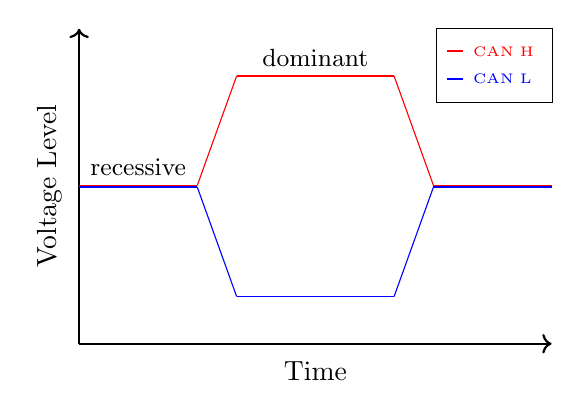
\begin{tikzpicture}
	%Draw axis
	\draw[thick,->] (0,0) -- coordinate (x axis mid) (6,0);
	\draw[thick,->] (0,0) -- coordinate (y axis mid) (0,4);
	%Draw axis label
	\node[below=0.1cm] at (x axis mid) {Time};
	\node[rotate=90, above=0.1cm] at (y axis mid) {Voltage Level};
	%Draw legend
	\matrix [draw,below left] at (current bounding box.north east) {
  		\draw[thick, red]  (0,0) -- (0.2,0) {} node[right]{\tiny CAN H}; \\
  		\draw[thick, blue] (0,0) -- (0.2,0){} node[right]{\tiny CAN L}; \\
	};

	%Draw CAN H
	\draw[red] (0,2.01)   -- (1.5,2.01) node[black, midway, above]{\small recessive};
	\draw[red] (1.5,2.01) -- (2,3.4);
	\draw[red] (2,3.4)    -- (4,3.4)    node[black, midway, above]{\small dominant};
	\draw[red] (4,3.4)    -- (4.5,2.01);
	\draw[red] (4.5,2.01) -- (6,2.01);
	%Draw CAN L
	\draw[blue] (0,1.99) -- (1.5,1.99);
	\draw[blue] (1.5,1.99) -- (2,0.6);
	\draw[blue] (2,0.6)    -- (4,0.6);
	\draw[blue] (4,0.6)    -- (4.5,1.99);
	\draw[blue] (4.5,1.99) -- (6,1.99);

	%
\end{tikzpicture}
\caption{CAN Physical Bit Transmission}
\label{fig:can_level}
\end{figure}

\subsection{Wiring and Bus Access}
\label{sec:wiring_access}

For wiring, a two-wire twisted pair cable with an impedance of 120$\Omega$ is used.
The topology is a line topology where stubs are allowed, but with a maximum length, depending on the bus speed.
On the first and last node of the bus line, terminating resistors with a value 120$\Omega$ avoid reflections on the bus line.
An example with two nodes is shown in \autoref{fig:can_wiring}.

\input{figures/can_wiring}

A CAN-transceiver, like shown in \autoref{fig:can_transceiver} connects the controller to the bus.
This transceiver converts the logic-level signals from the controller (CAN RX and CAN TX) to the bus levels and vice versa.
The dominant timeout protects the bus from a persistent dominant state in case of a faulty CAN controller.

\begin{figure}[htp]
\begin{circuitikz} \draw
	(4.5,3) node[op amp, rotate=180] (amp){}
	(amp.+) to [short,-o] ++(4, 0) node[right] {CAN H}
	(amp.-) to [short,-o] ++(4, 0) node[right] {CAN L}
	(2,3) node[invschmitt, rotate=180] (schm){}
	(amp.out) to (schm.in)
	(schm.out) to [short,-o] ++(-1, 0) node[left] {CAN RX}
	(8,5) node[pmos,emptycircle] (pmos){}
	(8,1) node[nmos] (nmos){}
	(8,0.5) node[ground] (gnd){}
	(8,6) node[vss, rotate = 180] (vss){}
	(pmos.S) to (vss)
	%(pmos.G) to [short] ++(-0.5,0)
	(pmos.D) to [short,-*] ++(0,-0.75)
	(nmos.D) to [short,-*] ++(0,0.75)
	(2.75,4.75)node[draw, minimum height=1cm, minimum width=2cm] (timeout) {\small Dominant Timeout}
	(5.75,4.75) node[draw, minimum height=1cm, minimum width=1.5cm] (driver) {\small Driver}
	(6.5,5) to (pmos.G)
	(6.5,4.5) to (7,4.5) to (7,1) to (nmos.G)
	(timeout) to (driver)
	(1,4.75) to [short,-o] ++(-0.75,0) node [left] {CAN TX}
	;
\end{circuitikz}
\caption{Simplified CAN Transceiver}
\label{fig:can_transceiver}
\end{figure}

The bitrate limit depends on the length of the bus \cite{TiCANPhy}.
However, the highest bitrate is limited to 1 Mbit per second for Classical CAN \cite{BoschCAN} and 8 Mbit for the data field of CAN Flexible Data-Rate (CAN FD)\cite{BoschCANFD}.
\autoref{tab:bus_speed} shows some example length and bitrate combinations for Classical CAN.
For CAN FD, the bitrate is only increased during the data field phase and could be eight times higher than the values in the table.

\begin{table}[ht]
	\centering
	\caption{Maximum bus speed}
	\begin{tabular}{|c|c|} 
		\hline
		Length & Max. Speed \\ \hline
		[m]    & [Kbps]     \\
		\hline
		\hline
		40     & 1000       \\ \hline
		100    & 500        \\ \hline
		200    & 250        \\ \hline
		500    & 100        \\ \hline
		1000   & 50         \\ \hline
	\end{tabular}
	\label{tab:bus_speed}
\end{table}

\FloatBarrier

\subsection{CAN Frames}
\label{sec:can_frames}

\begin{figure}[htp]
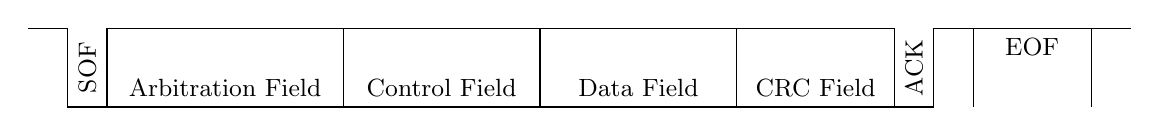
\begin{tikzpicture}
	%SOF
	\draw (0,1) -- ++(0.5,0) -- ++(0,-1) -- ++(0.5,0) -- ++(0,1);
	\node[rotate=90] at (0.75,0.5) {\small SOF};
	%Arbitration Field
	\draw (1,1) -- ++(3, 0);
	\draw (1,0) -- ++(3, 0) node[midway, above=0.25] {\small Arbitration Field};
	\draw (4, 0) -- ++(0,1);
	%Control Field
	\draw (4,1) -- ++(2.5, 0);
	\draw (4,0) -- ++(2.5, 0) node[midway, above=0.25] {\small Control Field};
	\draw (6.5, 0) -- ++(0,1);
	%Data Field
	\draw (6.5,1) -- ++(2.5, 0);
	\draw (6.5,0) -- ++(2.5, 0) node[midway, above=0.25] {\small Data Field};
	\draw (9, 0) -- ++(0,1);
	%CRC Field
	\draw (9,1) -- ++(2, 0);
	\draw (9,0) -- ++(2, 0) node[midway, above=0.25] {\small CRC Field};
	\draw (11, 0) -- ++(0,1);
	%ACK Field
	\draw (11,0) -- ++(0.5,0);
	\draw (11.5,0) -- ++(0,1);
	\node[rotate=90] at (11.25,0.5) {\small ACK};
	\draw (11.5,1) -- ++(0.5,0);
	\draw (12,0) -- ++(0,1);
	%EOF
	\draw (12,1) -- ++(1.5, 0) node[midway, below=0.25] {\small EOF};
	\draw (13.5, 0) -- ++(0,1);
	\draw (13.5,1) -- ++(0.5,0);

\end{tikzpicture}
\caption{CAN Frame Format}
\label{fig:can_frame_format}
\end{figure}

The Medium Access Control (MAC) specification defines the CAN frame format, as shown in \autoref{fig:can_frame_format}.
CAN uses so-called identifiers to identify the frames. Identifiers do not address nodes but identify the data that is being sent.
There are four basic frame formats. The "CAN Base Frame Format" with an 11-bit identifier; the "CAN Extended Frame Format" with a 29-bit identifier and their FD variants.
Frames start with the "Start of Frame" (SOF) bit. This bit is always dominant and signalizes the start of the frame and synchronizes the nodes.
The Arbitration Field includes the Base identifier and the "Remote Transmission Request" (RTR) bit in case of a basic frame.
For the extended frame format, the Identifier Extension (IDE) bit signalizes the identifier extension.
In this case, the IDE-bit and the remaining 18 bits of the identifier are also part of the Arbitration Field.
Nodes can use the RTR-bit to signal other nodes a request for transmission. For example, trigger a sensor read.

\begin{figure}[htp]
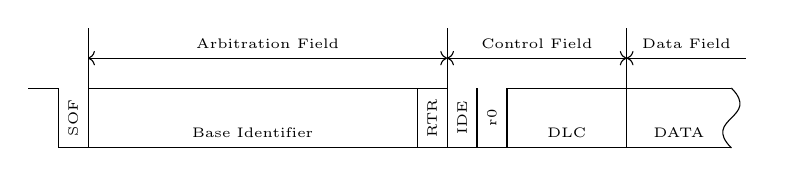
\begin{tikzpicture}[scale=0.76]
	%SOF
	\draw (0,1) -- ++(0.5,0) -- ++(0,-1) -- ++(0.5,0) -- ++(0,1);
	\node[rotate=90] at (0.75,0.5) {\tiny SOF};
	%Base Identifier
	\draw (1,1) -- ++(5.5, 0);
	\draw (1,0) -- ++(5.5, 0) node[midway, above=0.25] {\tiny Base Identifier};
	\draw (6.5, 0) -- ++(0,1);
	%RTR
	\draw (6.5, 0) -- ++(0.5,0);
	\draw (6.5, 1) -- ++(0.5,0);
	\draw (7, 0) -- ++(0,1);
	\node[rotate=90] at (6.75,0.5) {\tiny RTR};
	%IDE
	\draw (7, 0) -- ++(0.5,0);
	\draw (7.5, 0) -- ++(0,1);
	\node[rotate=90] at (7.25,0.5) {\tiny IDE};
	%r0
	\draw (7.5, 0) -- ++(0.5,0);
	\draw (8, 0) -- ++(0,1);
	\node[rotate=90] at (7.75,0.5) {\tiny r0};
	%DLC
	\draw (8,1) -- ++(2,0);
	\draw (8,0) -- ++(2,0) node[midway, above=0.25] {\tiny DLC};
	\draw (10, 0) -- ++(0,1);
	%data
	\draw (10,1) -- ++(1.75,0);
	\draw (10,0) -- ++(1.75,0) node[midway, above=0.25] {\tiny DATA};
	\draw (11.75,0) .. controls (11.25,0.5) and (12.25,0.5) .. (11.75,1);

	%Arbitration
	\draw (1,1) -- ++(0,1);
	\draw (7,1) -- ++(0,1);
	\draw[<->] (1,1.5) -- (7,1.5) node[midway, above] {\tiny Arbitration Field};
	%Control
	\draw (10,1) -- ++(0,1);
	\draw[<->] (7,1.5) -- (10,1.5) node[midway, above] {\tiny Control Field};
	%Data
	\draw[<-] (10,1.5) -- (12,1.5) node[midway, above] {\tiny Data Field};

\end{tikzpicture}
\caption{CAN Base Frame}
\label{fig:can_std_frame}
\end{figure}
\begin{figure}[htp]
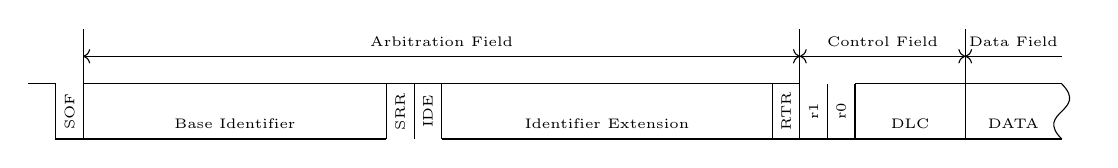
\begin{tikzpicture}[scale=0.7]
	%SOF
	\draw (0,1) -- ++(0.5,0) -- ++(0,-1) -- ++(0.5,0) -- ++(0,1);
	\node[rotate=90] at (0.75,0.5) {\tiny SOF};
	%Base Identifier
	\draw (1,1) -- ++(5.5, 0);
	\draw (1,0) -- ++(5.5, 0) node[midway, above=0.25] {\tiny Base Identifier};
	\draw (6.5, 0) -- ++(0,1);
	%SRR
	\draw (6.5, 1) -- ++(0.5,0);
	\draw (7, 0) -- ++(0,1);
	\node[rotate=90] at (6.75,0.5) {\tiny SRR};
	%IDE
	\draw (7, 1) -- ++(0.5,0);
	\draw (7.5, 0) -- ++(0,1);
	\node[rotate=90] at (7.25,0.5) {\tiny IDE};
	%Identifier Extension
	\draw (7.5,1) -- ++(6, 0);
	\draw (7.5,0) -- ++(6, 0) node[midway, above=0.25] {\tiny Identifier Extension};
	\draw (13.5, 0) -- ++(0,1);
	%RTR
	\draw (13.5,0) -- ++(0.5,0);
	\draw (13.5,1) -- ++(0.5,0);
	\draw (14,0) -- ++(0,1);
	\node[rotate=90] at (13.75,0.5) {\tiny RTR};
	%R1 R0
	\draw (14,0) -- ++(1,0);
	\draw (14.5,0) -- ++(0,1);
	\node[rotate=90] at (14.25,0.5) {\tiny r1};
	\draw (15,0) -- ++(0,1);
	\node[rotate=90] at (14.75,0.5) {\tiny r0};
	%DLC
	\draw (15,1) -- ++(2,0);
	\draw (15,0) -- ++(2,0) node[midway, above=0.25] {\tiny DLC};
	\draw (17, 0) -- ++(0,1);
	%Data
	\draw (17,1) -- ++(1.75,0);
	\draw (17,0) -- ++(1.75,0) node[midway, above=0.25] {\tiny DATA};
	\draw (18.75,0) .. controls (18.25,0.5) and (19.25,0.5) .. (18.75,1);
	
	%Arbitration
	\draw (1,1) -- ++(0,1);
	\draw (14,1) -- ++(0,1);
	\draw[<->] (1,1.5) -- (14,1.5) node[midway, above] {\tiny Arbitration Field};
	%Control
	\draw (17,1) -- ++(0,1);
	\draw[<->] (14,1.5) -- (17,1.5) node[midway, above] {\tiny Control Field};
	%Data
	\draw[<-] (17,1.5) -- ++(1.75,0) node[midway, above] {\tiny Data Field};
	
	\end{tikzpicture}
	\caption{CAN Extended Frame}
	\label{fig:can_ext_frame}
\end{figure}

\autoref{fig:can_std_frame} and \autoref{fig:can_ext_frame} shows examples for a Basic and Extended Frames.
CAN FD frames are outlined in more detail in the Bosch CAN FD specification \cite{BoschCANFD}.

In the Arbitration Field, collisions of multiple sending nodes are allowed.
The fact that a dominant bit always overrides a recessive bit resolves collisions in a way that the frame with the lowest identifier always wins.
Senders that want to write a recessive bit but get overridden by a dominant bit must abort their transmission silently.
Aborted frames can be retransmitted when the bus is in the idle state again.

The Control Field includes the reserved bit r0, the IDE, and the Data Length Code (DLC) for Basic frames and reserved bit r1, r0, and the DLC for Extended frames.
DLC indicates how many bytes are transmitted during the data phase.
\autoref{tab:dlc} lists the codes and number of bytes.
The maximum number of bytes for Classical CAN frames is eight, and the maximum number of bytes for CAN FD is 64.

\begin{table}
	\centering
	\caption{Data Length Codes}
	\begin{tabular}{|c|c|} 
		\hline
		DLC & Bytes \\
		\hline
		\hline
		0-8 & 0-8 \\ \hline
		9   & 12  \\ \hline
		10  & 16  \\ \hline
		11  & 20  \\ \hline
		12  & 24  \\ \hline
		13  & 32  \\ \hline
		14  & 48  \\ \hline
		15  & 64  \\ \hline
	\end{tabular}
	\label{tab:dlc}
\end{table}

The data field can be either empty or as many bytes as indicated by the DLC.

After the data field, the CRC field follows.
The length of the CRC field depends on the length of the data field.
A 15-bit CRC is used for all CAN frames up to eight data bytes.
For data field length up to 16 bytes, a 17-bit CRC is used.
A 21-bit CRC is used for a data field length of more than 16 bytes.
The CRC is calculated over the whole frame, from SOF to the end of the data field.

All nodes that received the frame correctly acknowledge their reception by putting a dominant bit into the ACK field.
The Field after the ACK field is the ACK-Delimiter and is always recessive.

EOF is the "End Of Frame". It is always seven recessive bits.
The Inter Frame Space is at least three recessive bits called Intermission.
Any node can override this Intermission with dominant bits to signal an Overload condition.

\begin{figure}[htp]
	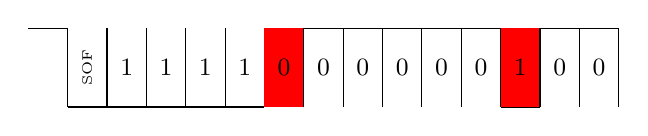
\begin{tikzpicture}[scale=1]
		\draw (0,1) -- ++(0.5,0);
		\foreach \x in {0.5,1,...,2.5}{
			\draw (\x,0) -- ++(0,1);
			\draw (\x,0) -- ++(0.5,0);
		}

		\node[rotate=90] at (0.75,0.5) {\tiny SOF};

		\foreach \x in {1,1.5,...,2.5}{
			\node[minimum height=1cm, minimum width=0.5cm] at (\x + 0.25,0.5) {\small 1};
		}

		%stuffing 1
		\draw (3,0) -- ++(0,1);
		\draw (3,1) -- ++(0.5,0);
		\node[fill=red, minimum height=1cm, minimum width=0.5cm] at (3.25,0.5) {\small 0};
		
		\foreach \x in {3.5,4,...,5.5}{
			\draw (\x,0) -- ++(0,1);
			\draw (\x,1) -- ++(0.5,0);
			\node[minimum height=1cm, minimum width=0.5cm] at (\x + 0.25,0.5) {\small 0};
		}
		
		%stuffing 2
		\draw (6,0) -- ++(0,1);
		\draw (6,0) -- ++(0.5,0);
		\node[fill=red, minimum height=1cm, minimum width=0.5cm] at (6.25,0.5) {\small 1};

		\foreach \x in {6.5,7}{
			\draw (\x,0) -- ++(0,1);
			\draw (\x,1) -- ++(0.5,0);
			\node[minimum height=1cm, minimum width=0.5cm] at (\x + 0.25,0.5) {\small 0};
		}
		\draw (7.5,0) -- ++(0,1);

	\end{tikzpicture}
	\caption{Bit Stuffing Example for 0x780 Identifier}
	\label{fig:can_stuffing}
\end{figure}

The bit-stuffing mechanism provides reliable synchronization during the transmission of the frame.
Five consecutive bits of the same value force a so-called stuffing bit.
The stuffing bit is a bit with the inverted value of the bits before and must be ignored by the receivers.
Stuffing bits change the length of the frame. An example is shown in \autoref{fig:can_stuffing}.
In the example stuffing bits, highlighted in red, extends the identifier field to 13 bits.
Additionally, it shows that SOF must be taken into account for stuffing.

Intentional violations of the stuffing rule are called Error Frames.
Overriding six consecutive bits with a dominant bit is an Error Active Frame.
Six recessive bits are called Error passive frame.
This rule allows signaling error conditions during all phases, including the EOF, in case of a CRC mismatch.

\FloatBarrier

\section{ISO-TP Transport Protocol}
\label{sec:iso_tp}

ISO-TP is a short name for the transport protocol specified in ISO15765 \cite{ISO15765}.
It specifies a transport protocol and network layer service operating in Controller Area Networks.
It was initially designed for road vehicle diagnostic services but it is not limited to them.
ISO-TP overcomes the limited frame size of CAN frames and allows us to send packets up to 4095 bytes and in the latest version extended to 4 gigabytes.
For this, the packets are segmented, transmitted in CAN frames, and reassembled on the receiver.
Additionally, a flow-control mechanism is defined to steer the timing of the frames.

The header data is called Process Control Information (PCI). The first nibble is the PCI-Type.
Following four PCI types are defined:
\begin{itemize}
	\item Single Frame
	\item First Frame
	\item Consecutive Frame
	\item Flow Control Frame
\end{itemize}

The rest of the PCI depends on the PCI-Type.
After the PCI, the rest of the frame is filled with payload data.
Single frames are used when the payload data plus one byte for the PCI  fits into a single CAN frame.
For Classical CAN, it is a payload length of seven bytes. For CAN FD, it can be up to 63 bytes.
The other three PCI types are used for payload lengths larger than a single frame can carry.

A segmented packet starts with a "First Frame" (FF) from the sender to the receiver.
The First Frame contains information about the total payload data length.
The receiver sends back a "Flow Control" frame (FC).
This FC frame can either signal "Continue To Send", "Wait", or that the packet would "Overflow" the receiver.
Furthermore, the FC frame contains a Block Size (BS) and Minimal Separation Time (ST\textsubscript{min}).
When the FC frame is of type CTS, the sender continues with sending "Consecutive Frames" (CF).
When BS is zero, the sender sends as many CF frames as needed to transfer the payload data.
Otherwise, the sender has to stop after BS CF frames and wait for another FC frame.
ST\textsubscript{min} defines a minimum separation time between two frames.
A ST\textsubscript{min} of zero is allowed.
If the receiver answers with an FC-Frame with the Flow-State OVFLW, the sender has to abort the transmission.
In case the sender does not receive an FC-Frame within one second, it aborts the transmission.
The Flow-State WAIT causes a reset of the sender timeout.
Receivers cancel the reception of the packet when no CF frame is received within one second.

\autoref{fig:iso_tp_sequence} shows an example sequence with a BS of three.

\input{figures/iso_tp_sequence.tex}

\begin{table}
	\centering
	\caption{ISO-TP Protocol Control Information}
	\begin{tabular}{|c|c|c|c|c|c|c|c|c|c|} \hline
	Byte:                 & \multicolumn{2}{c|}{0}              & \multirow{2}{*}{1}  & \multirow{2}{*}{2} & \multirow{2}{*}{3} & \multirow{2}{*}{4} & \multirow{2}{*}{5} & \multirow{2}{*}{6} & \multirow{2}{*}{7} \\ \cline{2-3}
	                      & 7..4               & 3..0           &                     &                    &                    &                    &                    &                    &                    \\ \hline \hline
	\multirow{2}{*}{SF}   & \multirow{2}{*}{0} & SF\_DL         & data 0              & data 1             & data 2             & data 3             & data 4             & data5              & data 6             \\ \cline{3-10}
	                      &                    & 0              & SF\_DL              & data 0             & data 1             & data 2             & data 3             & data 4             & data 5             \\ \hline
	\multirow{2}{*}{FF}   & \multirow{2}{*}{1} & \multicolumn{2}{c|}{FF\_DL}          & data 0             & data 1             & data 2             & data 3             & data 4             & data 5             \\ \cline{3-10}
	                      &                    & \multicolumn{2}{c|}{0}               & \multicolumn{4}{c|}{FF\_DL}                                                       & data 0             & data 1             \\ \hline
	CF                    & 2                  & SN             & data 0              & data 1             & data 2             & data 3             & data 4             & data 5             & data 6             \\ \hline
	FC                    & 3                  & FS             & BS                  & STmin              & \multicolumn{5}{c|}{}                                                                                  \\ \hline
	\end{tabular}
	\label{tab:pci}
\end{table}

\begin{table}
	\centering
	\caption{Flow-States}
	\begin{tabular}{|l|c|} \hline
	Type  & Number \\ \hline \hline
	CTS   (Continue To Send)  & 0      \\ \hline
	WAIT  (Wait)              & 1      \\ \hline
	OVFLW (Overflow)          & 2      \\ \hline
	\end{tabular}
	\label{tab:fs}
\end{table}

\autoref{tab:pci} shows examples of classical CAN frames with all PCI types.
Elements labeled with data 0 to data 6 are payload data.

\newpage

SF is the Single Frame and has the PCI-type-number 0.
For Single Frames with maximum payload data size of seven bytes, the Single Frame data length (SF\_DL) is encoded in bit zero to three of the first PCI byte.
CAN FD frames can have a frame data length up to 64 bytes in a single frame. Single frames with more than seven bytes of data encode the data length in the second PCI byte.

FF is the First Frame and has the PCI-type-number 1.
The data length (FF\_DL) of the packet is encoded in byte zero and byte one of the PCI.
Byte one is the lower octet, and bit zero to bit 3 of byte 0 contains the upper nibble of the 12-bit data length.
For a data length bigger than 4095 bytes, bit zero to three of byte zero and byte one is set to zero.
The data length is then encoded in byte two to five.

CFs are Consecutive Frames, containing payload data and a sequence number (SN).
The PCI-type-number is 2, and the sequence number is located at the lower nibble of byte zero.
The sequence number is a counter that is set to one for the first CF and incremented by one for every frame and wraps around at 15.
When the sequence number wraps around, it starts with zero again.
The sequence number is used to detect out of order or lost frames.

FCs are Frame Control Frames and have the PCI-type-number 3.
The lower 4-bit nibble of the first byte contains Flow State. The numbers are shown in \autoref{tab:fs}.
The second byte, Block-Size (BS), defines how many CF frames the sender is allowed to transmit until he has to wait for an FC-Frame again.

\FloatBarrier

\section{IPv6}
\label{sec:ipv6}

\begin{table}
	\centering
	\caption{Internet Protocol Suite}
	\begin{tabular}{|c|l|l|} \hline
	Layer                         & Example                      \\ \hline \hline
	Application                   & HTTP, HTTPS, CoAP, MQTT      \\ \hline
	Transport                     & TCP, UDP                     \\ \hline
	\cellcolor{black!10} Internet & IPv4, IPv6, ICMP             \\ \hline
	Link                          & Ethernet, IEEE 802.15.4, CAN \\ \hline
	\end{tabular}
	\label{tab:ips}
\end{table}

IP (Internet Protocol) covers the Internet layer of the Internet Protocol Suite (\autoref{tab:ips}) \cite{rfc1122}.
Internet Protocol version six (IPv6) was first introduced in RFC2460 \cite{rfc2460} as an RFC Draft-Standard in December 1998
and got finally standardized with RFC8200 \cite{rfc8200} in July 2017.
It solves some problems from its predecessor, the Internet Protocol version four (IPv4) \cite{rfc791}.

The most significant improvements are:

\begin{itemize}
	\item Extended address range (from 32 bits to 128-bits)
	\item Stateless Address Autoconfiguration
	\item Simplification of the header
	\item Use of Neighbor Discovery protocol
	\item Next header instead of header options
\end{itemize}

RFC8200 defines some important terminologies:
A "node" is a device with an IPv6 stack.
"Link" refers to the lowest layer defined in \autoref{tab:ips}, and
"interface" is the node's attachment to a link.

\subsection{IPv6 Addresses}
\label{sec:ipv6_addr}

IPv6 addresses are written in a hexadecimal representation of 16-bit blocks, separated by colons.
Leading zeros can be omitted, and all zero blocks can be written as two colons (::).
The all-zero blocks can span more than a single 16-bit block, but can only be used once in a representation.
RFC5952 \cite{rfc5952} describes the recommended text representation of IPv6 addresses.

For example, the address fe80:0000:0000:0000:0000:00ff:fe00:1234 can be written as fe80::ff:fe00:1234

An IPv6 address prefix can be written as \textit{IPv6-address/prefix-length}.
For example fe80::00ff:fe00:1234/64 is interpreted as fe80:000:0000:0000 address prefix.

\begin{table}
	\centering
	\caption{IPv6 Address Types}
	\begin{tabular}{|l|l|l|} \hline
	Type                & Prefix            \\ \hline \hline
	Unspecified Address & ::/128 (all zero) \\ \hline
	Loopback            & ::1/128           \\ \hline
	Multicast           & FF00::/8          \\ \hline
	Link-Local Unicast  & FE80::/10         \\ \hline
	Global Unicast      & everything else   \\ \hline
	\end{tabular}
	\label{tab:ipv6_addr_types}
\end{table}

RFC4291 \cite{rfc4291} defines five types of addresses, identified by their higher-order bits.
The address types are shown in \autoref{tab:ipv6_addr_types}.

\begin{figure}[htp]
	\begin{center}
	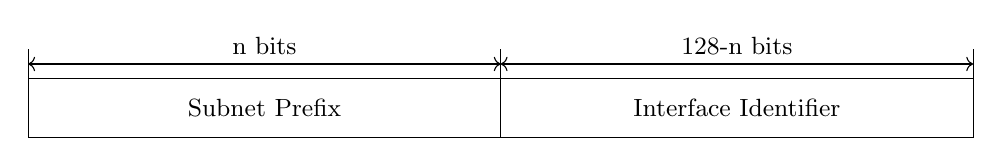
\begin{tikzpicture}[scale=0.75]
		\draw (0,0) rectangle (16,1);
		\draw (0,1) -- ++(0,0.5);
		\draw (8,0) -- ++(0,1.5);
		\draw (16,1) -- ++(0,0.5);
		\node at (4, 0.5) {\small Subnet Prefix};
		\node at (12, 0.5) {\small Interface Identifier};
		\draw[<->] (0,1.25) -- (8,1.25) node[midway, above] {\small n bits};
		\draw[<->] (8,1.25) -- (16,1.25) node[midway, above] {\small 128-n bits};
	\end{tikzpicture}
	\end{center}
	\caption{Subnet Prefix of an IPv6 address}
	\label{fig:ipv6_subnet_prefix}
\end{figure}

Unicast IPv6 addresses can generally be treated as if they have no internal structure.
Nevertheless, more sophisticated nodes may be aware of subnets, which logically group addresses.
\autoref{fig:ipv6_subnet_prefix} shows how the address is split into the subnet prefix and an Interface Identifier (IID).
Routers, for example, can use subnets to create hierarchical boundaries.
The IID needs to be unique within the subnet and identifies an interface on a link (lowest layer on \autoref{tab:ips}).
All Unicast addresses not starting with the binary value 000 must have an IID according to the Modified EUI-64 format with a length of 64 bits.
Addresses of this format can be derived from the link-address as described in RFC4291 \cite{rfc4291} Appendix A.
If the address is derived, for example, from an Ethernet MAC address, it has a universal scope and is globally unique.
IIDs derived from link addresses that are not globally unique must be unique in the local scope.

\begin{figure}[htp]
	\begin{center}
	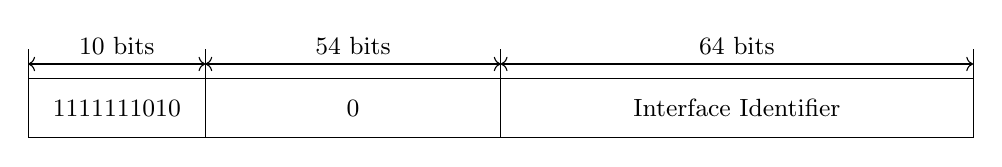
\begin{tikzpicture}[scale=0.75]
		\draw (0,0) rectangle (16,1);
		\draw (0,1) -- ++(0,0.5);
		\draw (3,0) -- ++(0,1.5);
		\draw (8,0) -- ++(0,1.5);
		\draw (16,1) -- ++(0,0.5);
		\node at (1.5, 0.5) {\small 1111111010};
		\node at (5.5, 0.5) {\small 0};
		\node at (12, 0.5) {\small Interface Identifier};
		\draw[<->] (0,1.25) -- (3,1.25) node[midway, above] {\small 10 bits};
		\draw[<->] (3,1.25) -- (8,1.25) node[midway, above] {\small 54 bits};
		\draw[<->] (8,1.25) -- (16,1.25) node[midway, above] {\small 64 bits};
	\end{tikzpicture}
	\end{center}
	\caption{Link Local Unicast address}
	\label{fig:ipv6_ll_unicast}
\end{figure}

An interface can have several addresses, but must at least have one Link-Local Unicast address.
The Link-Local Unicast address is formed as shown in \autoref{fig:ipv6_ll_unicast}.

\begin{figure}[htp]
	\begin{center}
	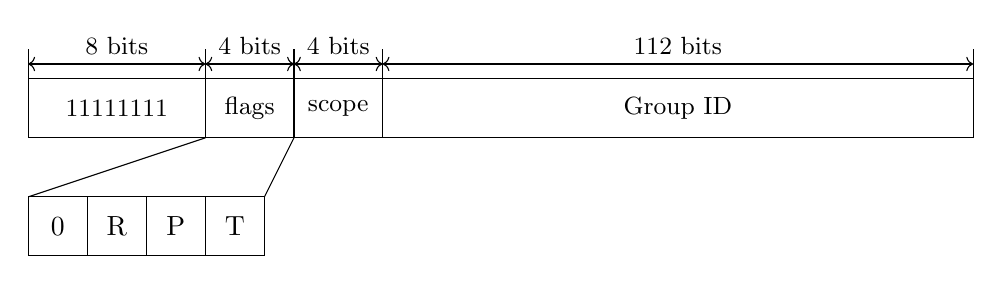
\begin{tikzpicture}[scale=0.75]
		\draw (0,2) rectangle (16,3);
		\draw (0,3) -- ++(0,0.5);
		\draw (3,2) -- ++(0,1.5);
		\draw (4.5,2) -- ++(0,1.5);
		\draw (6,2) -- ++(0,1.5);
		\draw (16,3) -- ++(0,0.5);
		\node at (1.5, 2.5) {\small 11111111};
		\node at (3.75, 2.5) {\small flags};
		\node at (5.25, 2.5) {\small scope};
		\node at (11, 2.5) {\small Group ID};
		\draw[<->] (0,3.25) -- ++(3,0) node[midway, above] {\small 8 bits};
		\draw[<->] (3,3.25) -- ++(1.5,0) node[midway, above] {\small 4 bits};
		\draw[<->] (4.5,3.25) -- ++(1.5,0) node[midway, above] {\small 4 bits};
		\draw[<->] (6,3.25) -- (16,3.25) node[midway, above] {\small 112 bits};

		\draw (3,2) -- (0,1);
		\draw (4.5,2) -- (4,1);
		\draw (0,0) rectangle (4,1);
		\node at (0.5,0.50) {0};
		\draw (1,0) -- ++(0,1);
		\node at (1.5,0.50) {R};
		\draw (2,0) -- ++(0,1);
		\node at (2.5,0.50) {P};
		\draw (3,0) -- ++(0,1);
		\node at (3.5,0.50) {T};
	\end{tikzpicture}
	\end{center}
	\caption{Multicast address}
	\label{fig:ipv6_multicast_addr}
\end{figure}

\begin{table}
	\centering
	\caption{Multicast Scopes}
	\begin{tabular}{|c|l|} \hline
	Number & Scope              \\ \hline \hline
	0      & reserved           \\ \hline
	1      & Interface-Local    \\ \hline
	2      & Link-Local         \\ \hline
	3      & reserved           \\ \hline
	4      & Admin-Local        \\ \hline
	5      & Site-Local         \\ \hline
	6-7    & unassigned         \\ \hline
	8      & Organization-Local \\ \hline
	9-D    & unassigned         \\ \hline
	E      & Global             \\ \hline
	F      & reserved           \\ \hline
	\end{tabular}
	\label{tab:mcast_scopes}
\end{table}

The multicast address format depicted in \autoref{fig:ipv6_multicast_addr}.
The highest byte is the multicast prefix 0xff, followed by four bits flags, and four bits scope.
For the flags, only the T flag is of interest in this work.
The T-flag signals an unassigned address when it's set to one.
If the T-flag is zero, the address is a "well-known" address.
The scopes are listed in \autoref{tab:mcast_scopes}.

\newpage

Some predefined multicast addresses are, for example:
\begin{itemize}
	\item ff01::1 Interface-Local All-Nodes multicast address
	\item ff02::1 Link-Local All-Nodes multicast address
	\item ff02::2 Link-Local All-Routers multicast address
	\item ff02::2 Site-Local All-Routers multicast address
	\item ff02:0:0:0:0:1:ffXX:XXXX Solicited-Node multicast address
\end{itemize}
The Solicited-Node multicast address is formed by the prefix ff02:0:0:0:0:1:ff::/104 concatenated with the low-order 24 bits of the unicast or anycast address.

\begin{figure}[htp]
	\begin{center}
	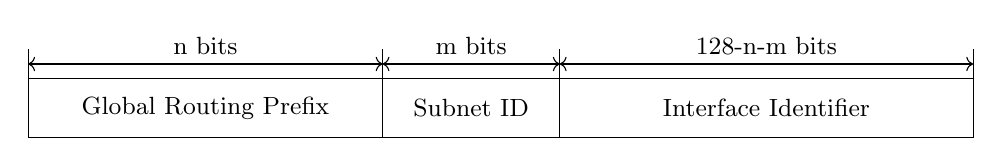
\begin{tikzpicture}[scale=0.75]
		\draw (0,0) rectangle (16,1);
		\draw (0,1) -- ++(0,0.5);
		\draw (6,0) -- ++(0,1.5);
		\draw (9,0) -- ++(0,1.5);
		\draw (16,1) -- ++(0,0.5);
		\node at (3, 0.5) {\small Global Routing Prefix};
		\node at (7.5, 0.5) {\small Subnet ID};
		\node at (12.5, 0.5) {\small Interface Identifier};
		\draw[<->] (0,1.25) -- (6,1.25) node[midway, above] {\small n bits};
		\draw[<->] (6,1.25) -- (9,1.25) node[midway, above] {\small m bits};
		\draw[<->] (9,1.25) -- (16,1.25) node[midway, above] {\small 128-n-m bits};
	\end{tikzpicture}
	\end{center}
	\caption{Global Unicast address}
	\label{fig:ipv6_global_unicast}
\end{figure}

A Global Unicast Address, as shown in \autoref{fig:ipv6_global_unicast} consists of a global routing prefix, a subnet ID, and the IID.
Global unicast addresses not starting with binary 000 always have an IID length of 64 bytes, same as the Link-Local Unicast address.
The global routing prefix is a value assigned to a site and distributed by the routers on that site.
The Subnet ID is an identifier of a link within the site.
The global unicast address is used to address single nodes that are not Link-Local, for example, a node on the internet.

A node must at least listen to the following addresses:
\begin{itemize}
	\item The Link-Local addresses assigned to the interfaces
	\item The loopback address
	\item The All-Nodes multicast address
	\item The Solicited-Nodes multicast address for each anycast and multicast address
	\item All multicast addresses for multicast groups the node has joined
\end{itemize}

\subsection{IPv6 Header}
\label{sec:ipv6_hdr}
\begin{figure}[htp]
	\begin{center}
	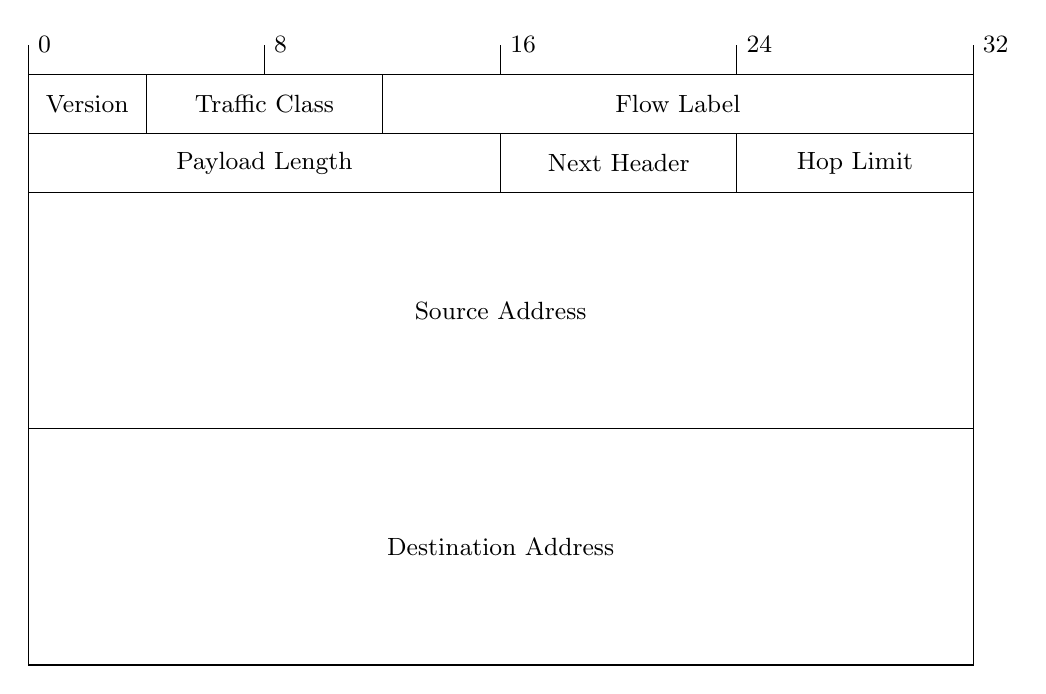
\begin{tikzpicture}[scale=0.75]
		\draw (0,0) -- (16,0) -- (16,10) -- (0,10) -- cycle;
		\draw (0,9) -- (16,9);
		\draw (0,8) -- (16,8);
		\draw (0,4) -- (16,4);
		\draw (0,10) -- ++(0,0.5) node[right] {\small 0};
		\draw (4,10) -- ++(0,0.5) node[right] {\small 8};
		\draw (8,10) -- ++(0,0.5) node[right] {\small 16};
		\draw (12,10) -- ++(0,0.5) node[right] {\small 24};
		\draw (16,10) -- ++(0,0.5) node[right] {\small 32};

		\draw (2,10) -- (2,9);
		\node at (1,9.5) {\small Version};
		\draw (6,10) -- (6,9);
		\node at (4, 9.5) {\small Traffic Class};
		\node at (11, 9.5) {\small Flow Label};

		\draw (8,9) -- (8,8);
		\node at (4, 8.5) {\small Payload Length};
		\draw (12,9) -- (12,8);
		\node at (10, 8.5) {\small Next Header};
		\node at (14,8.5) {\small Hop Limit};

		\node at (8, 6) {\small Source Address};
		\node at (8, 2) {\small Destination Address};
	\end{tikzpicture}
	\end{center}
	\caption{IPv6 Header}
	\label{fig:ipv6_hdr}
\end{figure}

The IPv6 header, as shown in \autoref{fig:ipv6_hdr}, has a fixed size of 40 bytes.
The fixed length makes it easier to process IPv6 headers and allows simple compression schemes like IPHC \cite{rfc6282}.

The 4-bit Version field is always 0x6 for IPv6.
Traffic-Class has a length of eight bits where the six most significant bits correspond to the Differentiated Service (DS) \cite{rfc2474} and
the remaining two bits are used for Explicit Congestion Notification (ECN) \cite{rfc3168}.
The 16-bit Payload Length field is an unsigned integer, defining the remaining length of the packet.
This number excludes the IP header but includes all possible next headers.
The next header field identifies the header type of the following extension- or protocol-header, if any, or "No Next Header" (59) if there aren't any.

The concept of Next Headers instead of options makes IPv6 very flexible.
Any number of options headers may follow the IPv6 header in a chained manner.
Therefor, every option header includes another next header field, forming a chain until the next header is an upper-layer protocol or the "No Next Header" option.

The Hop Limit is a counter, initialized by the node that issued the packet, with the desired limit of how many times this packet may be forwarded.
Every hop that forwards, a router, for example, decrements the hop limit by one.
When the limit reaches zero, the packet is discarded, and the node sends a message back to the source to inform about the discarding.

The Source Address is the IP address of the interface, and the Destination Address is the IP address of the desired receiver.
The Source Address and Destination Address both have a length of 128 bits.

IPv6 supports fragmentation, where a packet is cut into smaller fragments at the sender, transported, and reassembled at the destination.
For fragmentation, the Fragment Header is used.
Packet fragmentation is only allowed at the sender. Routers are not allowed to fragment packets.
IPv6 requires a minimal Maximum Transfer Unit (MTU) of 1280 bytes, which is the minimum link MTU that must be supported by every node on the internet.
Links that are not capable of transferring packets of at last 1280 bytes must apply fragmentation and reassembly at the Data-Link Layer.

\subsection{ICMPv6}
\label{sec:icmp_v6}

\begin{figure}[htp]
	\begin{center}
	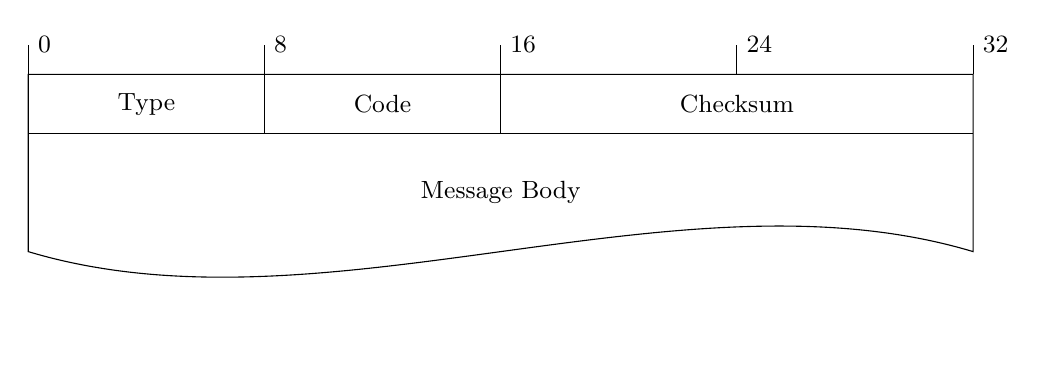
\begin{tikzpicture}[scale=0.75]
		\draw (0,0) .. controls (5, -1.5) and (11,1.5) .. (16,0) -- (16,3) -- (0,3) -- cycle;
		\draw (0,3) -- ++(0,0.5) node[right] {\small 0};
		\draw (4,3) -- ++(0,0.5) node[right] {\small 8};
		\draw (8,3) -- ++(0,0.5) node[right] {\small 16};
		\draw (12,3) -- ++(0,0.5) node[right] {\small 24};
		\draw (16,3) -- ++(0,0.5) node[right] {\small 32};

		\draw (4,2) -- ++(0,1);
		\node at (2,2.5) {\small Type};
		\draw (8,2) -- ++(0,1);
		\node at (6, 2.5) {\small Code};
		\node at (12, 2.5) {\small Checksum};
		\draw (0,2) -- ++(16,0);

		\node at (8,1) {\small Message Body};
	\end{tikzpicture}
	\end{center}
	\caption{Internet Control Message Protocol Format}
	\label{fig:icmp_format}
\end{figure}

\begin{table}
	\centering
	\caption{ICMPv6 Types defined by RFC4443}
	\begin{tabular}{|c|l|l|} \hline
	Type & Name                    & Description \\ \hline \hline
	1    & Destination Unreachable & \makecell[l]{Packet cannot be delivered to \\ its destination}                                  \\ \hline
	2    & Packet Too Big          & \makecell[l]{Router cannot forward the packet \\ because it exceeds a link-MTU}                 \\ \hline
	3    & Time Exceeded           & \makecell[l]{Router received a packet with a \\ hop-limit of zero or decremented \\ it to zero} \\ \hline
	4    & Parameter Problem       & \makecell[l]{Node detected a problem on a header \\ field that cannot be resolved}              \\ \hline
	128  & Echo Request            & A request to reply back to the sender                                                           \\ \hline
	129  & Echo Reply              & The reply to the Echo request                                                                   \\ \hline
	\end{tabular}
	\label{tab:ipv6_icmp_types}
\end{table}

ICMPv6 is a Transport-Layer protocol defined in \cite{rfc4443}.
\autoref{fig:icmp_format} depicts the ICMPv6 header format.
\autoref{tab:ipv6_icmp_types} shows ICMPv6 Types defined directly by the ICMPv6 RFC.
Other types are defined in the respective RFCs defining ICMPv6 messages.

\subsection{Neighbor Discovery Protocol}
\label{sec:ipv6_ndp}

\begin{figure}[htp]
	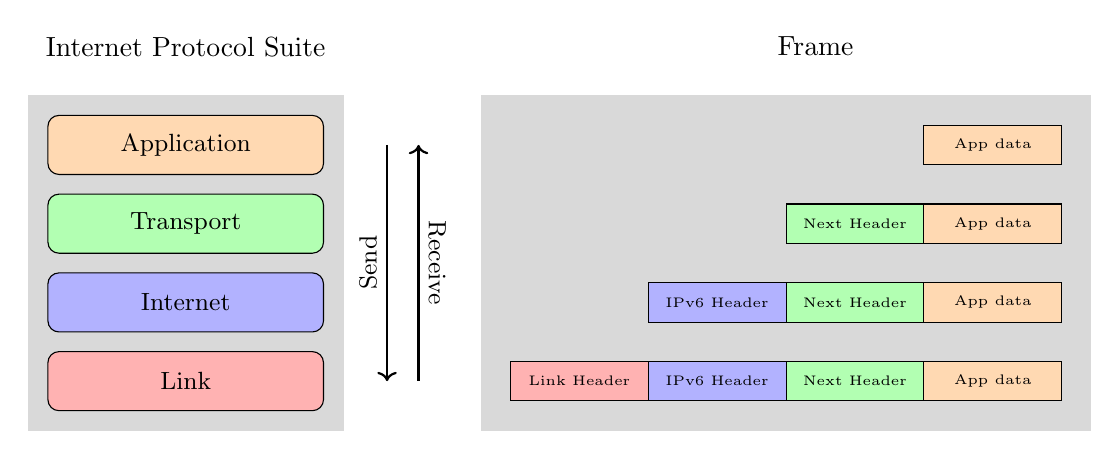
\begin{tikzpicture}[
		psuite/.style={
			draw=black,
			rounded corners,
			rectangle, 
			minimum width=3.5cm,
			minimum height=0.75cm,
			font=\small},
		frame/.style= {
			draw=black,
			rectangle, 
			minimum width=1.75cm,
			minimum height=0.5cm,
			font=\tiny}]
		\node (app) [psuite, fill=orange!30] {Application};
		\node [right of=app, xshift=9.25cm, frame, fill=orange!30] {App data};
		\node (transp) [below of=app, psuite, fill=green!30] {Transport};
		\node [right of=transp, xshift=9.25cm, frame, fill=orange!30] {App data};
		\node [right of=transp, xshift=7.5cm, frame, fill=green!30] {Next Header};
		\node (inet) [below of=transp, psuite, fill=blue!30] {Internet};
		\node [right of=inet, xshift=9.25cm, frame, fill=orange!30] {App data};
		\node [right of=inet, xshift=7.5cm, frame, fill=green!30] {Next Header};
		\node [right of=inet, xshift=5.75cm, frame, fill=blue!30] {IPv6 Header};
		\node (link) [below of= inet, psuite, fill=red!30] {Link};
		\node [right of=link, xshift=9.25cm, frame, fill=orange!30] {App data};
		\node [right of=link, xshift=7.5cm, frame, fill=green!30] {Next Header};
		\node [right of=link, xshift=5.75cm, frame, fill=blue!30] {IPv6 Header};
		\node [right of=link, xshift=4cm, frame, fill=red!30] {Link Header};

		\draw [thick, ->]($(app.east) + (0.8cm,0)$) -- ($(link.east) + (0.8cm,0)$) node[midway, above = 0.1, rotate=90] {\small Send};
		\draw [thick, <-]($(app.east) + (1.2cm,0)$) -- ($(link.east) + (1.2cm,0)$) node[midway, above = 0.1, rotate=270] {\small Receive};

		\node [above of=app, yshift=0.25cm] {Internet Protocol Suite};
		\node [above of=app, yshift=0.25cm, xshift=8cm] {Frame};

		\begin{scope}[on background layer]
			\fill [black!15] ($(app.north west) + (-0.25cm, 0.25)$) rectangle ($(link.south east)+ (0.25cm, -0.25)$);
			\fill [black!15] ($(app.north) + (3.75cm, 0.25)$) rectangle ($(link.south)+ (11.5cm, -0.25)$);
		\end{scope}

	\end{tikzpicture}
	\caption{IPv6 Header Encapsulation}
	\label{fig:ipv6_encapsulation}
\end{figure}


\autoref{fig:ipv6_encapsulation} shows how the data and headers of the upper layers get encapsulated in an IPv6 datagram that gets finally encapsulated in a frame.
IPv6 works on 128-bit addresses, but nodes use different addresses on their Link-Layer to transmit the frames.
This so-called Link-Layer address could either be the address of the receiver directly on the link or the Link-Layer address of the router
in case the receiver is not in the same Link-Local network.
The Link-Layer address of the next hop or the destination, in case of a Link-Local transfer, needs to be discovered first.
IPv6 uses the Link-Layer Neighbor Discovery protocol (NDP) \cite{rfc4861} for this task.
NDP packets are encapsulated in ICMPv6 (Internet Control Message Protocol) messages.
The nodes use a so-called Neighbor Cache to learn the relevant addresses of its neighborhood.
Addresses that have been resolved once stay in the cache for a predefined time.
For this time, the address does not need to be resolved but can be taken from the cache.

\begin{figure}[htp]
	\begin{center}
	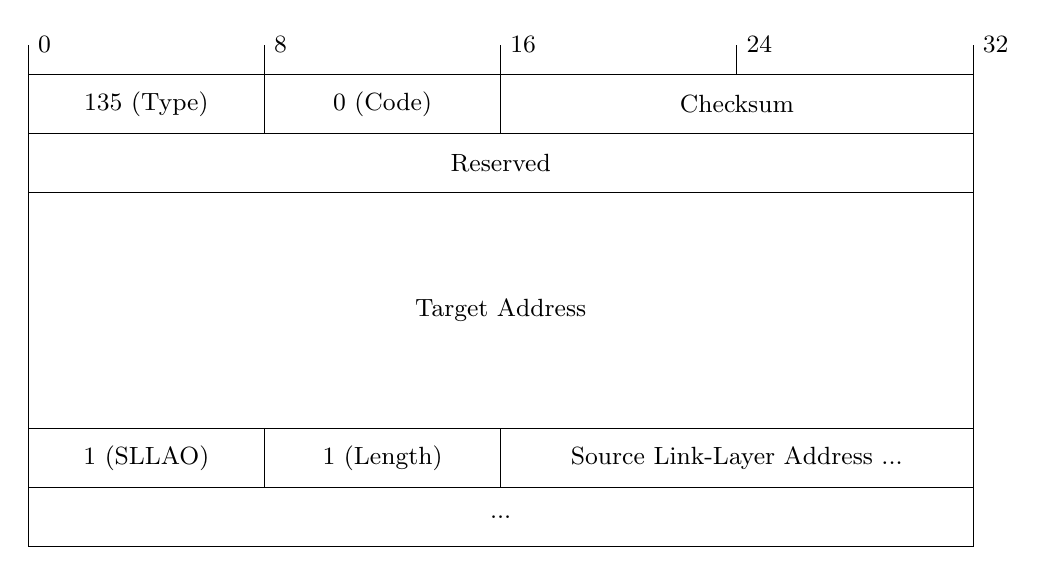
\begin{tikzpicture}[scale=0.75]
		\draw (0,0) -- (16,0) -- (16,8) -- (0,8) -- cycle;
		\draw (0,8) -- ++(0,0.5) node[right] {\small 0};
		\draw (4,8) -- ++(0,0.5) node[right] {\small 8};
		\draw (8,8) -- ++(0,0.5) node[right] {\small 16};
		\draw (12,8) -- ++(0,0.5) node[right] {\small 24};
		\draw (16,8) -- ++(0,0.5) node[right] {\small 32};

		\draw (4,8) -- (4,7);
		\node at (2,7.5) {\small 135 (Type)};
		\draw (8,8) -- (8,7);
		\node at (6, 7.5) {\small 0 (Code)};
		\node at (12, 7.5) {\small Checksum};
		\draw (0,7) -- ++(16,0);

		\node at (8, 6.5) {\small Reserved};
		\draw (0,6) -- ++(16,0);

		\node at (8, 4) {\small Target Address};
		\draw (0,2) -- ++(16,0);
		
		\draw (4,2) -- (4,1);
		\node at (2,1.5) {\small 1 (SLLAO)};
		\draw (8,2) -- (8,1);
		\node at (6, 1.5) {\small 1 (Length)};
		\node at (12, 1.5) {\small Source Link-Layer Address ...};
		\draw (0,1) -- ++(16,0);
		\node at (8, 0.5) {\small ...};

	\end{tikzpicture}
	\end{center}
	\caption{Neighbor Solicitation Message Example}
	\label{fig:ipv6_ns}
\end{figure}
\input{figures/ipv6_ndp_na}

NDP defines two message formats for finding direct neighbors.
\begin{itemize}
	\item Neighbor Solicitation Message Format
	\item Neighbor Advertisement Message Format
\end{itemize}

\newpage

Neighbor Advertisement messages propagate a node's Link-Layer address to other nodes.
They are broadcasted when the node joins a network or can be requested by a Neighbor Solicitation message (NS).
NAs not requested by an NS are called unsolicited advertisements and typically sent to the all-node multicast address.
The node can send an NA message to the solicited-node multicast address and wait for an NA from the targeted node to resolve an address.
The node can send an NS message to the targeted nodes unicast address to check if the node is still available.

\autoref{fig:ipv6_ns} shows an example of a Neighbor Solicitation message.
The ICMPv6 Type of an NS is 135, and the code is always zero for an NS message.
The Target Address field contains the IPv6 address of the node, where the NA should be requested.
The Target Address is followed by the option field.
In case the source of the IP header is not the unspecified address (::), the option field must include the Source Link-Layer Address option (SLLAO).
The length field of a Link-Layer Address Option (LLAO) describes the total length of the option field in eight-bytes units.
For example, if the Link-Layer address has a length of six bytes or smaller, the length field is one.

The answer to an NS message is the Neighbor Advertisement message (NA).
\autoref{fig:ipv6_na} depicts an example of such an NA message.
The ICMPv6 type field is always 136, and the code is always zero for an NA message.
The R-bit implies that the node, sending the NA, is a router.
A set S-bit means that the NA message is sent as a response to an NS message.
The O-bit indicates that this NA message should override a possibly cached Link-Layer address from a previously sent NA.
The Target Address can either be the address of the solicitation node or the all-nodes multicast address in case of an unsolicited NA or an unspecified source address.

\begin{figure}[htp]
	\begin{center}
	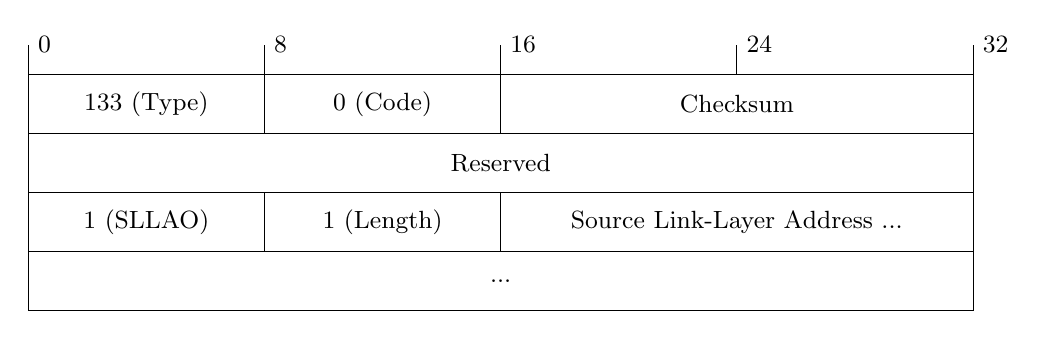
\begin{tikzpicture}[scale=0.75]
		\draw (0,0) rectangle (16,4);
		\draw (0,4) -- ++(0,0.5) node[right] {\small 0};
		\draw (4,4) -- ++(0,0.5) node[right] {\small 8};
		\draw (8,4) -- ++(0,0.5) node[right] {\small 16};
		\draw (12,4) -- ++(0,0.5) node[right] {\small 24};
		\draw (16,4) -- ++(0,0.5) node[right] {\small 32};

		\draw (4,4) -- (4,3);
		\node at (2,3.5) {\small 133 (Type)};
		\draw (8,4) -- (8,3);
		\node at (6, 3.5) {\small 0 (Code)};
		\node at (12, 3.5) {\small Checksum};
		\draw (0,3) -- ++(16,0);

		\node at (8, 2.5) {\small Reserved};
		\draw (0,2) -- ++(16,0);

		\draw (4,2) -- (4,1);
		\node at (2,1.5) {\small 1 (SLLAO)};
		\draw (8,2) -- (8,1);
		\node at (6, 1.5) {\small 1 (Length)};
		\node at (12, 1.5) {\small Source Link-Layer Address ...};
		\draw (0,1) -- ++(16,0);
		\node at (8, 0.5) {\small ...};

	\end{tikzpicture}
	\end{center}
	\caption{Router Solicitation Message Example}
	\label{fig:ipv6_rs}
\end{figure}
\begin{figure}[htp]
	\begin{center}
	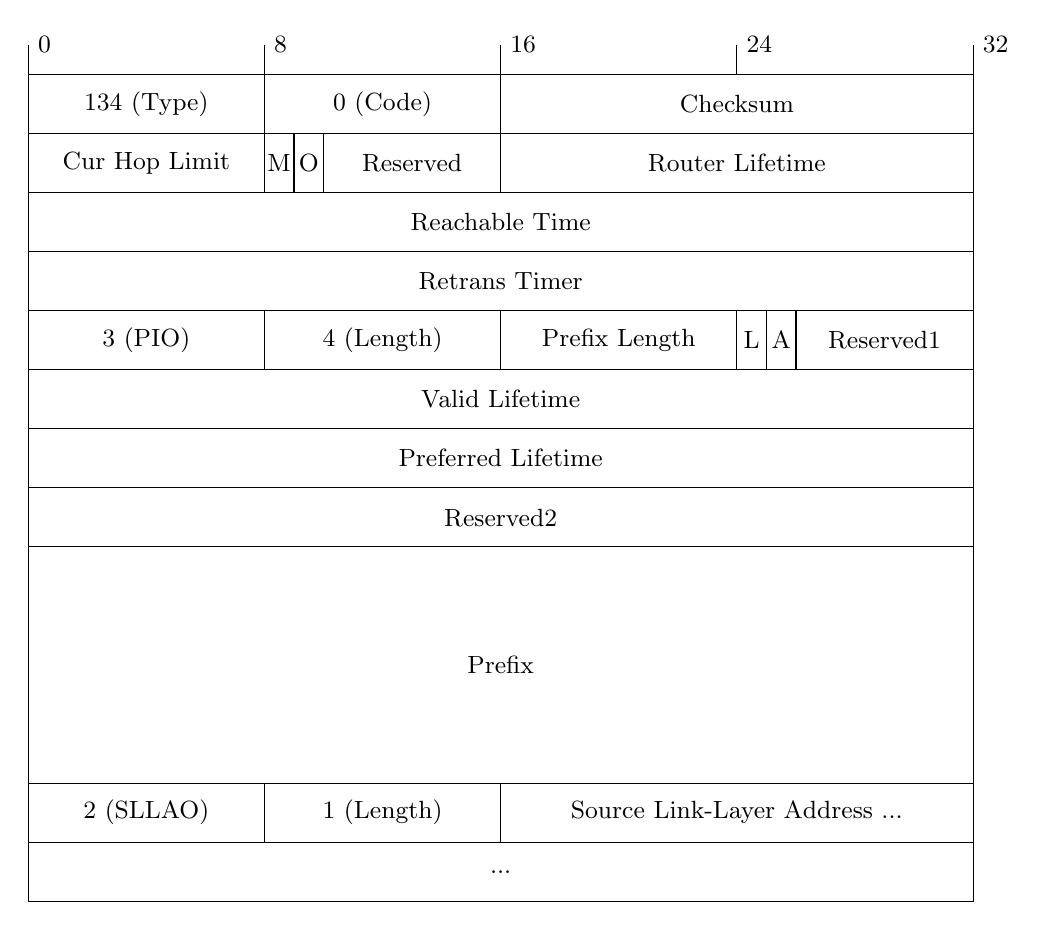
\begin{tikzpicture}[scale=0.75]
		\draw (0,0) rectangle (16,14);
		\draw (0,14) -- ++(0,0.5) node[right] {\small 0};
		\draw (4,14) -- ++(0,0.5) node[right] {\small 8};
		\draw (8,14) -- ++(0,0.5) node[right] {\small 16};
		\draw (12,14) -- ++(0,0.5) node[right] {\small 24};
		\draw (16,14) -- ++(0,0.5) node[right] {\small 32};
0
		\draw (4,13) -- ++(0,1);
		\node at (2,13.5) {\small 134 (Type)};
		\draw (8,13) -- ++(0,1);
		\node at (6, 13.5) {\small 0 (Code)};
		\node at (12, 13.5) {\small Checksum};
		\draw (0,13) -- ++(16,0);

		\draw (4,12) -- ++(0,1);
		\node at (2, 12.5) {\small Cur Hop Limit};
		\draw (4.5,12) -- ++(0,1);
		\node at (4.25, 12.5) {\small M};
		\draw (5,12) -- ++(0,1);
		\node at (4.75, 12.5) {\small O};
		\draw (8,12) -- ++(0,1);
		\node at (6.5, 12.5) {\small Reserved};
		\node at (12, 12.5) {\small Router Lifetime};
		\draw (0,12) -- ++(16,0);

		\node at (8, 11.5) {\small Reachable Time};
		\draw (0,11) -- ++(16,0);

		\node at (8, 10.5) {\small Retrans Timer};
		\draw (0,10) -- ++(16,0);

		\draw (4,9) -- ++(0,1);
		\node at (2,9.5) {\small 3 (PIO)};
		\draw (8,9) -- ++(0,1);
		\node at (6, 9.5) {\small 4 (Length)};
		\draw (12,9) -- ++(0,1);
		\node at (10, 9.5) {\small Prefix Length};
		\draw (12.5,9) -- ++(0,1);
		\node at (12.25, 9.5) {\small L};
		\draw (13,9) -- ++(0,1);
		\node at (12.75, 9.5) {\small A};
		\node at (14.5, 9.5) {\small Reserved1};
		\draw (0,9) -- ++(16,0);

		\node at (8,8.5) {\small Valid Lifetime};
		\draw (0,8) -- ++(16,0);
		\node at (8,7.5) {\small Preferred Lifetime};
		\draw (0,7) -- ++(16,0);
		\node at (8,6.5) {\small Reserved2};
		\draw (0,6) -- ++(16,0);
		\node at (8,4) {\small Prefix};
		\draw (0,2) -- ++(16,0);

		\draw (4,2) -- (4,1);
		\node at (2,1.5) {\small 2 (SLLAO)};
		\draw (8,2) -- (8,1);
		\node at (6, 1.5) {\small 1 (Length)};
		\node at (12, 1.5) {\small Source Link-Layer Address ...};
		\draw (0,1) -- ++(16,0);
		\node at (8, 0.5) {\small ...};

	\end{tikzpicture}
	\end{center}
	\caption{Router Advertisement Message Example}
	\label{fig:ipv6_ra}
\end{figure}

NDP defines two message formats for finding routers on the link.
\begin{itemize}
	\item Router Solicitation Message Format
	\item Router Advertisement Message Format
\end{itemize}

Router advertisement messages (RA) propagate information about routers on the link.
Unsolicited router advertisements are sent out to the all-nodes multicast address by the routers periodically.
A node can also request a router advertisement by sending out a Router Solicitation (RS) message to the all-routers multicast group.
The router will then answer with an RA to the issuer's unicast address.
The RS message is shown in \autoref{fig:ipv6_rs}.

The RA message is shown in \autoref{fig:ipv6_ra}.
The ICMPv6 Type of an RA is 134, and the code is always zero for an RA message.
The Current Hop Limit field tells the receiving node which hop-limit should be used for outgoing packets.
Zero means unspecified. The M and O flags are DHCPv6 related and not relevant for this work.
The Router Lifetime field is an unsigned 16-bit value in units of a second. It specifies the lifetime associated with the default router.
The Reachable Time specifies a time interval in milliseconds for which a node can assume that an already discovered node is still reachable.
The last timer field, the Retrans Timer, defines the time between the retransmission of a Neighbor Solicitation message in units of milliseconds.
The RA example has two option fields included. The Prefix Info and the SLLAO.
The SLLAO includes the source Link-Layer address like the RS message.
The Prefix Info option (PIO) tells the receiving node information about the prefix used for address autoconfiguration.
The length value indicates the number of bits used as the prefix. The prefix is always in the upper address bytes since the address
in this option has the same length ass an entire address.
The L-Flag indicates that the prefix is on-link, which means that it can be reached directly without any router involved.
The A-Flag signals the prefix can be used for Stateless Address Autoconfiguration.
Valid Lifetime and Preferred Lifetime signal the SLAAC for how long the address is valid and for how long it should be used.
All-ones (0xffffffff) values signal infinite lifetime.

\subsection{Stateless Address Autoconfiguration}
\label{sec:ipv6_slaac}

\begin{figure}[htp]
	\begin{center}
	\begin{tikzpicture}[scale=0.45, node distance=2cm, every node/.append style={scale=0.45}]
		\node (start) [startstop] {Interface up};
		\node (ll_ten) [process, below = of start] {Create tentative Link-Local address};
		\node (dad_ns) [io, below = of ll_ten] {Send NS message with tentative Link-Local address (DAD)};
		\node (dad_na) [io, below = of dad_ns] {Wait for NA message with tentative Link-Local address (DAD) or Timeout};
		\node (dad) [decision, below = of dad_na] {NA message received?};
		\node (alt_addr) [decision, right of=dad, xshift=7cm] {Alternative address?};
		\node (dad_fail) [startstop, below = of alt_addr] {DAD failed};
		\node (ll) [process, below = of dad] {Apply Link-Local address};
		\node (rs) [io, below = of ll] {Send RS};
		\node (ra) [io, below = of rs] {Wait for RA};
		\node (glob_create) [process, below = of ra] {Create tentative global address};
		\node (dad_ns_glob) [io, below = of glob_create] {Send NS message with global address from RA prefix (DAD)};
		\node (dad_na_glob) [io, below = of dad_ns_glob] {Wait for NA message with global address from RA prefix (DAD) or Timeout};
		\node (dad_glob) [decision, below = of dad_na_glob] {NA message received?};
		\node (glob) [process, below = of dad_glob] {Apply global address};

		\draw [arrow] (start) -- (ll_ten);
		\draw [arrow] (ll_ten) -- (dad_ns);
		\draw [arrow] (dad_ns) -- (dad_na);
		\draw [arrow] (dad_na) -- (dad);
		\draw [arrow] (dad) -- node [anchor=south] {yes (DAD failed)} (alt_addr);
		\draw [arrow] (dad) -- node [anchor=east] {no (DAD succeeded)} (ll);
		\draw [arrow] (alt_addr) |- node [anchor=south] {yes} (ll_ten);
		\draw [arrow] (alt_addr) -- node [anchor=east] {no} (dad_fail);
		\draw [arrow] (ll) -- (rs);
		\draw [arrow] (rs) -- (ra);
		\draw [arrow] (ra) -- (glob_create);
		\draw [arrow] (glob_create) -- (dad_ns_glob);
		\draw [arrow] (dad_ns_glob) -- (dad_na_glob);
		\draw [arrow] (dad_na_glob) -- (dad_glob);
		\draw [arrow] (dad_glob) -- node [anchor=east] {no (DAD succeeded)} (glob);
		\coordinate [right = of ra] (ra_right) ;
		\draw [arrow] (dad_glob.east) -- ++(2cm,0) node [anchor=south] {yes (DAD failed)} -|   (ra_right) -- (ra.east);
		\draw [arrow] (glob.south) -- ++(0,-1cm) -| (ra_right) -- (ra);
	\end{tikzpicture}
	\end{center}
	\caption{Stateless Address Autoconfiguration}
	\label{fig:ipv6_slaac}
\end{figure}

IPv6 nodes use the Stateless Address Autoconfiguration (SLAAC), defined in RFC4862 \cite{rfc4862}, to configure  the interface's addresses.
The SLAAC mechanism generates Link-Local and global addresses.
The Link-Local address is formed by combining the Link-Local prefix with the IID, and global addresses use the prefix
learned from RA messages, combined with the IID.
\autoref{fig:ipv6_slaac} shows the routine to perform SLAAC.
When an interface is initialized, it assigns itself a tentative Link-Local address, formed as described above.
Then the node sends out an NS message with the Target Address of the tentatively chosen address.
The source IPv6 address is the unspecified address (::) and the destination IPv6 address is the solicited multicast address.
This process is called Duplicate Address Detection (DAD).
If there is a node on the link, using the same address, it returns an NA message, indicating a duplication, and the node then discards
the tentative address and depending on the configuration, generates a new address.
After the DAD, the node has a Link-Local address assigned and can send an RS.
All routers in the network answer the RS with an RA message where the node can get the prefix information from.
With this prefix information, the node forms a global address and starts listening to that address.

\FloatBarrier

\section{6lo}
\label{sec:6lo}

\begin{figure}[htp]
	\begin{tikzpicture}[
		layer/.style={
			minimum width=13cm,
			text width=13cm,
			minimum height=1.5cm,
			fill=black!5,
			align=left,
			node distance=0,
			font=\small},
		example/.style={
				draw=black,
				fill=white,	
				rectangle, 
				minimum width=2.5cm,
				minimum height=0.75cm,
				font=\small},
		node distance=0.25cm and 1cm]
\begin{scope}[on background layer]
		\node (app) [layer] {Application};
		\node (transp) [below = of app, layer] {Transport};
		\node (inet) [below = of transp, layer] {Internet};
		\node (link) [below = of inet, yshift=-0.5cm,layer] {Link};
		\node at (link) (adapt)  [fill=green!20, text width=9cm, minimum height=1cm, align=left, xshift=-2cm, yshift=0.85cm] {6lo Adaption};
\end{scope}
		\node (app_http) [right of = app, xshift=-2.5cm, example] {HTTP};
		\node (app_coap) [right = of app_http, example] {CoAP};
		\node (app_mqtt) [right = of app_coap, example] {MQTT};
		\node (transp_udp) [right of = transp, xshift=-2.5cm, example] {UDP};
		\node (transp_tcp) [right = of transp_udp, example] {TCP};
		\node (transp_icmp) [right = of transp_tcp, example] {ICMPv6};
		\node (inet_ipv6) [right of = inet, xshift=1cm, example, minimum width=9cm] {IPv6};
		\node (link_wpan) [right of = link, xshift=-2.5cm, example] {802.15.4};
		\node (link_can) [right = of link_wpan, example] {CAN};
		\node (adapt_6lowpan) [above = of  link_wpan, yshift=-0.2cm, example] {6LoWPAN};
		\node (adapt_6locan) [above = of link_can, yshift=-0.2cm, example] {6LoCAN};
		\node (link_eth) [right = of link_can, example] {Ethernet};
	\end{tikzpicture}
	\caption{6lo Adaption layer example}
	\label{fig:6lo_layer}
\end{figure}


6lo is the name of an Internet Engineering Task Force (IETF) Working Group (WG).
The 6lo WG focus on IPv6 connectivity over constrained nodes.
The nodes are constrained in the sense of limited power, memory, and lack of some required Link-Layer services.
The WG is working on IPv6-over-foo adaption layers, using specifications from 6LoWPAN technologies like RFC4944 \cite{rfc4944} and RFC6282 \cite{rfc6282}.
6lo technologies usually have a 6lo adaption-layer, as shown in \autoref{fig:6lo_layer}.

\subsection{IP Header Compression}
\label{sec:iphc}

For this document, the concept of the Adaption layer and the IP Header Compression (IPHC) is of importance.
The IPHC reduces redundant information in the 40 bytes IPv6 header.
The payload length, for example, is usually known from the Link-Layer packet size and is therefore always elided.
The version field is also always elided because the compression is only defined for IPv6.
Fields that can be recovered from Link-Layer information can be fully elided.
Fields filled with default parameters can either be entirely elided or chosen on a set of default values.
On a Link-Layer where the Interface Identifier (IID) is generated from the Link-Layer address,
the IPv6 header with a Link-Local source and Link-Local destination address, the IPv6 addresses in the header are
redundant and can be reconstructed from the Link-Layer headers.
This saves up to 38 bytes of data.
The compression can either be stateless or context-based.
A context is a global routing prefix that is known by all nodes and has an index.
This 4-bit index can then be used instead of transmitting the 64-bit prefix.
The distribution of the contexts is out of scope and not defined by aby standard yet.

\begin{figure}[htp]
	\begin{center}
	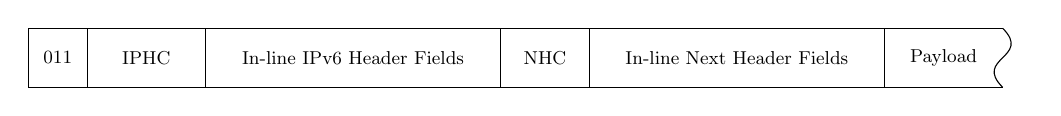
\begin{tikzpicture}[scale=0.75, every node/.append style={scale=0.75}]
		\draw (0,0) -- ++(16.5,0);
		\draw (0,1) -- ++(16.5,0);
		\draw (0,0) -- ++(0,1);
		\draw (16.5,0) .. controls (16,0.5) and (17,0.5) .. (16.5,1);

		\draw (1,0) -- ++(0,1);
		\node at (0.5, 0.5) {\small 011};

		\draw (3,0) -- ++(0,1);
		\node at (2, 0.5) {\small IPHC};

		\draw (8,0) -- ++(0,1);
		\node at (5.5, 0.5) {\small In-line IPv6 Header Fields};

		\draw (9.5,0) -- ++(0,1);
		\node at (8.75, 0.5) {\small NHC};

		\draw (14.5,0) -- ++(0,1);
		\node at (12, 0.5) {\small In-line Next Header Fields};

		\node at (15.5, 0.5) {\small Payload};
	\end{tikzpicture}
	\end{center}
	\caption{IPHC Frame Format}
	\label{fig:6lo_iphc_frame}
\end{figure}

The IPHC dispatch is a bit-field at the beginning of a packet, as shown in \autoref{fig:6lo_iphc_frame}.
The dispatch signals a IPHC compressed packet.
IPv6 header fields that cannot be fully elided are carried in-line after the IPHC bit-field.
The order of the in-lined data follows the order of the IPHC bit-field from left to right.
If the Next Header is compressible, the Next Header Compression (NHC) field follows the In-Line Header Fields.
Next-Header fields that cannot be fully elided, follow the NHC.

\begin{figure}[htp]
	\begin{center}
	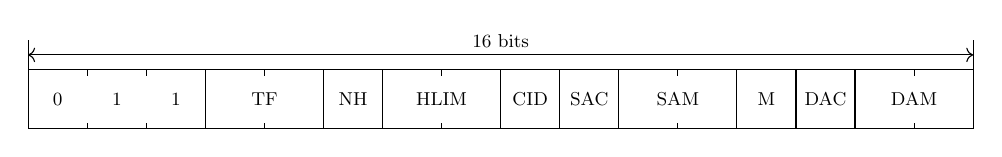
\begin{tikzpicture}[scale=0.75, every node/.append style={scale=0.75}]
		\draw (0,0) rectangle (16,1);
		\draw (0,1) -- ++(0,0.5);
		\draw (16,1) -- ++(0,0.5);
		\draw[<->] (0,1.25) -- (16,1.25) node[midway, above] {\small 16 bits};

		\foreach \x in {1,2,...,15}{
			\draw (\x,1) -- ++(0,-0.1);
			\draw (\x,0) -- ++(0,0.1);
		}

		\draw (3,0) -- ++(0,1);
		\node at (0.5, 0.5) {\small 0};
		\node at (1.5, 0.5) {\small 1};
		\node at (2.5, 0.5) {\small 1};

		\draw (5,0) -- ++(0,1);
		\node at (4, 0.5) {\small TF};

		\draw (6,0) -- ++(0,1);
		\node at (5.5, 0.5) {\small NH};

		\draw (8,0) -- ++(0,1);
		\node at (7, 0.5) {\small HLIM};

		\draw (9,0) -- ++(0,1);
		\node at (8.5, 0.5) {\small CID};

		\draw (10,0) -- ++(0,1);
		\node at (9.5, 0.5) {\small SAC};

		\draw (12,0) -- ++(0,1);
		\node at (11, 0.5) {\small SAM};

		\draw (13,0) -- ++(0,1);
		\node at (12.5, 0.5) {\small M};

		\draw (14,0) -- ++(0,1);
		\node at (13.5, 0.5) {\small DAC};

		\node at (15, 0.5) {\small DAM};

	\end{tikzpicture}
	\end{center}
	\caption{IPHC Format}
	\label{fig:6lo_iphc}
\end{figure}

The IPHC bit-field, including the three-bit dispatch (011), has a length of 16 bits, as shown in \autoref{fig:6lo_iphc}.

TF (Traffic-Class, Flow Label):\\
The first two bits define the Traffic-Class and Flow Label compression (TF).
The meaning of the values is stated in \autoref{tab:6lo_tf}.

\begin{table}[h!]
	\centering
	\caption{Traffic-Class and Flow-Label Compression}
	\begin{tabular}{|c|l|} \hline
	Code & Description                                           \\ \hline \hline
	00   & ECN + DSCP + 4-bit Pad + Flow Label (4 bytes)           \\ \hline
	01   & ECN + 2-bit Pad + Flow Label (3 bytes), DSCP is elided. \\ \hline
	10   & ECN + DSCP (1 byte), Flow Label is elided.              \\ \hline
	11   & Traffic-Class and Flow-Label are elided.                \\ \hline
	\end{tabular}
	\label{tab:6lo_tf}
\end{table}

NH (Next Header):\\
When this bit is set, the next header field is compressed, and the LOWPAN\_NHC (Next header compression) is following the in-line field.
Otherwise, the Next header byte is carried in-line.

HLIM (Hop Limit):\\
The HLIM field defines the compressed Hop Limit.

\begin{table}[h!]
	\centering
	\caption{Hop Limit Compression}
	\begin{tabular}{|c|l|} \hline
	Code & Description \\ \hline \hline
	00   & No compression. Carried in-line \\ \hline
	01   & The hop limit is 1              \\ \hline
	10   & The hop limit is 64             \\ \hline
	11   & The hop limit is 255            \\ \hline
	\end{tabular}
	\label{tab:6lo_hlim}
\end{table}

CID (Context Identifier Extension):\\
If set, an 8-bit Context Identifier is carried in-line. The format is shown in \autoref{fig:6lo_cid}.
If a context-based compression is used for source or destination-address, context zero is used.

\begin{figure}[htp]
	\begin{center}
	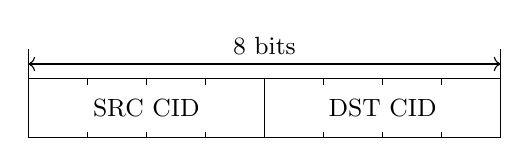
\begin{tikzpicture}[scale=0.75]
		\draw (0,0) rectangle (8,1);
		\draw (0,1) -- ++(0,0.5);
		\draw (8,1) -- ++(0,0.5);
		\draw[<->] (0,1.25) -- (8,1.25) node[midway, above] {\small 8 bits};

		\foreach \x in {1,2,...,7}{
			\draw (\x,1) -- ++(0,-0.1);
			\draw (\x,0) -- ++(0,0.1);
		}

		\draw (4,0) -- ++(0,1);
		\node at (2, 0.5) {\small SRC CID};
		\node at (6, 0.5) {\small DST CID};
	\end{tikzpicture}
	\end{center}
	\caption{Context ID Format}
	\label{fig:6lo_cid}
\end{figure}

SAC (Source Address Compression):\\
If set, the source address compression is context-based.
If not, it is stateless.

SAM (Source Address Mode):\\
The source address compression mode is interpreted differently for context-based or stateless compression.

The enumeration for stateless source address compression is shown in \autoref{tab:6lo_SAM_0}.
\begin{table}[h!]
	\centering
	\caption{Stateless Source and Destination-Address Compression}
	\begin{tabular}{|c|l|c|} \hline
	Code & Description                                           & In-lined bits\\ \hline \hline
	00   & No compression. Address is carried in-line            & 128 \\ \hline
	01   & \makecell[l]{The Prefix is fe80::/64.\\
	                    The IID is carried in-line}              & 64  \\ \hline
	10   & \makecell[l]{The Prefix is fe80::ff:fe00:XXXX/112.\\
	                    The last 16 bits are carried in-line}    & 16  \\ \hline
	11   & \makecell[l]{The Prefix is fe80::/64.\\
			    The IID is reconstructed from the\\
			    Link-Layer address.}                     & 0   \\ \hline
	\end{tabular}
	\label{tab:6lo_SAM_0}
\end{table}

The enumeration for context-based source address compression is shown in \autoref{tab:6lo_SAM_1}.
\begin{table}[h!]
	\centering
	\caption{Context-Based Source- and Destination-Address Compression}
	\begin{tabular}{|c|l|c|} \hline
	Code & Description                                                  & In-lined bits\\ \hline \hline
	00   & The unspecified address ::                                   & 0  \\ \hline
	01   & \makecell[l]{The Prefix is taken from the context. \\
	                    The IID is carried in-line.}                    & 64 \\ \hline
	10   & \makecell[l]{The Prefix is taken from the context. \\
			    Bits not covered by the context are \\
			    filled with ::ff:fe00:XXXX.\\
			    The last 16 bits are carried in-line}           & 16 \\ \hline
	11   & \makecell[l]{The Prefix is taken from the context.\\
			    The IID is reconstructed from the Link-Layer \\
			    address, if not covered by the context.}        & 0 \\ \hline
	\end{tabular}
	\label{tab:6lo_SAM_1}
\end{table}

M (Multicast Compression):\\
If set, the destination address is a multicast address.

DAC (Destination Address Compression):\\
If set, the destination address compression is context-based.
If not, it is stateless.

DAM (Destination Address Mode):\\
The interpretation of the destination address compression mode depends on the combination of multicast compression and destination address compression.

The enumeration for stateless non-multicast compression is shown in table \autoref{tab:6lo_SAM_0} and is the same as the compression for the source address.

The enumeration for context-based destination address compression is the same as the compression for the source address,
with the exception that case 00 is not allowed, and is shown in \autoref{tab:6lo_SAM_1}.

The enumeration for stateless multicast destination address compression is shown in 

\begin{table}[h!]
	\centering
	\caption{Stateless Multicast Destination-Address Compression}
	\begin{tabular}{|c|l|c|} \hline
	Code & Description                                   & In-lined bits\\ \hline \hline
	00   & No compression. Address is carried in-line    & 128 \\ \hline
	01   & The address takes the form ffXX::XX:XXXX:XXXX & 48  \\ \hline
	10   & The address takes the form ffXX::XX:XXXX      & 32  \\ \hline
	11   & The address takes the form ff02::XX           & 8   \\ \hline
	\multicolumn{3}{l}{Bytes marked as XX are carried in-line.}\\
	\end{tabular}
	\label{tab:6lo_DAC_M}
\end{table}

\begin{figure}[htp]
	\begin{center}
	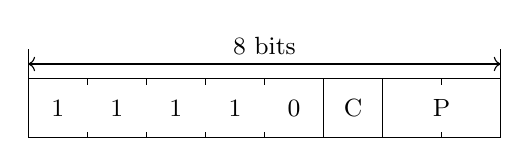
\begin{tikzpicture}[scale=0.75]
		\draw (0,0) rectangle (8,1);
		\draw (0,1) -- ++(0,0.5);
		\draw (8,1) -- ++(0,0.5);
		\draw[<->] (0,1.25) -- (8,1.25) node[midway, above] {\small 8 bits};

		\foreach \x in {1,2,...,7}{
			\draw (\x,1) -- ++(0,-0.1);
			\draw (\x,0) -- ++(0,0.1);
		}
		\foreach \x in {0.5,1.5,...,3.5}{
			\node at (\x, 0.5) {\small 1};
		}

		\node at (4.5, 0.5) {\small 0};
		\draw (5,0) -- ++(0,1);
		\node at (5.5, 0.5) {\small C};
		\draw (6,0) -- ++(0,1);
		\node at (7, 0.5) {\small P};
	\end{tikzpicture}
	\end{center}
	\caption{Next Header Compression for UDP Headers}
	\label{fig:6lo_nhc_udp}
\end{figure}

Another significant compression is the Next Header Compression, specifically the UDP header compression.
The format is shown in \autoref{fig:6lo_nhc_udp}. The first five bits are the dispatch for UDP header compression.

C (Checksum):
If C is set, the Checksum of the UDP datagram is elided or carried in-line otherwise.

P (Ports):
The enumeration of the port compression is shown in \autoref{tab:6lo_DAC}

\begin{table}[h!]
	\centering
	\caption{Stateless Multicast Destination Address Compression}
	\begin{tabular}{|c|l|c|} \hline
	Code & Description                                            & In-lined bits\\ \hline \hline
	00   & No compression. Both ports are carried in-line         & 32 \\ \hline
	01   & \makecell[l]{Source-Port fully in-lined.\\
	                    Destination port takes the form 0xf0XX}   & 24  \\ \hline
	10   & \makecell[l]{Destination Port fully in-lined.\\
	                    Source port takes the form 0xf0XX}        & 24  \\ \hline
	11   & Source- and Destination Port take the form 0xf0bX      & 8   \\ \hline
	\multicolumn{3}{l}{Bytes marked as XX are carried in-line.}\\
	\end{tabular}
	\label{tab:6lo_DAC}
\end{table}

\begin{figure}[htp]
	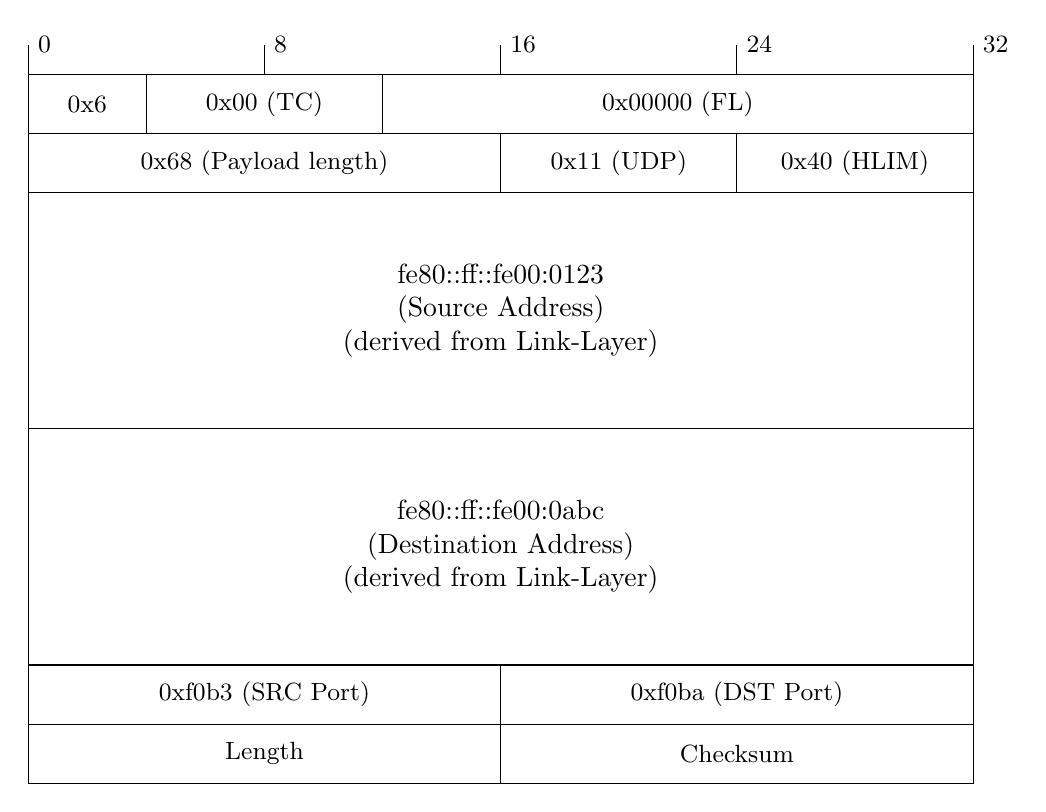
\begin{tikzpicture}[scale=0.75]
		%IPv6
		\draw (0,0) rectangle (16,12);
		\draw (0,11) -- (16,11);
		\draw (0,10) -- (16,10);
		\draw (0,6) -- (16,6);
		\draw (0,2) -- (16,2);
		\draw (0,1) -- (16,1);

		\draw (0,12) -- ++(0,0.5) node[right] {\small 0};
		\draw (4,12) -- ++(0,0.5) node[right] {\small 8};
		\draw (8,12) -- ++(0,0.5) node[right] {\small 16};
		\draw (12,12) -- ++(0,0.5) node[right] {\small 24};
		\draw (16,12) -- ++(0,0.5) node[right] {\small 32};

		\draw (2,12) -- ++(0,-1);
		\node at (1,11.5) {\small 0x6};
		\draw (6,12) -- ++(0,-1);
		\node at (4, 11.5) {\small 0x00 (TC)};
		\node at (11, 11.5) {\small 0x00000 (FL)};

		\draw (8,11) -- ++(0,-1);
		\node at (4, 10.5) {\small 0x68 (Payload length)};
		\draw (12,11) -- ++(0,-1);
		\node at (10, 10.5) {\small 0x11 (UDP)};
		\node at (14,10.5) {\small 0x40 (HLIM)};

		\node at (8, 8) [align=center] {fe80::ff::fe00:0123 \\(Source Address) \\ (derived from Link-Layer)};
		\node at (8, 4) [align=center] {fe80::ff::fe00:0abc \\ (Destination Address) \\ (derived from Link-Layer)};

		\draw (8,2) -- ++(0,-1);
		\node at (4,1.5) {\small 0xf0b3 (SRC Port)};
		\node at (12,1.5) {\small 0xf0ba (DST Port)};

		\draw (8,1) -- ++(0,-1);
		\node at (4,0.5) {\small Length};
		\node at (12,0.5) {\small Checksum};

	\end{tikzpicture}\\
	\vspace{2em}
	48 bytes from the original header result in following 4 bytes:\\
	\vspace{2em}
	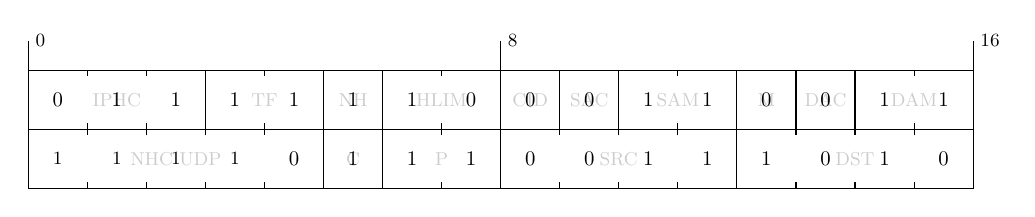
\begin{tikzpicture}[scale=0.75, every node/.append style={scale=0.75}]
		%IPHC
		\draw (0,0) rectangle (16,2);
		\draw (0,1) -- (16,1);
		\draw (0,2) -- ++(0,0.5) node[right] {\small 0};
		\draw (8,2) -- ++(0,0.5) node[right] {\small 8};
		\draw (16,2) -- ++(0,0.5) node[right] {\small 16};

		\foreach \x in {1,2,...,15}{
			\draw (\x,2) -- ++(0,-0.1);
			\draw (\x,1) -- ++(0,0.1);
			\draw (\x,1) -- ++(0,-0.1);
			\draw (\x,0) -- ++(0,0.1);
		}

		\draw (3,1) -- ++(0,1);
		\node at (1.5, 1.5) {\color{black!20}\small IPHC};
		\node at (0.5, 1.5) {0};
		\node at (1.5, 1.5) {1};
		\node at (2.5, 1.5) {1};

		\draw (5,1) -- ++(0,1);
		\node at (4, 1.5) {\color{black!20}\small TF};
		\node at (3.5, 1.5) {1};
		\node at (4.5, 1.5) {1};

		\draw (6,1) -- ++(0,1);
		\node at (5.5, 1.5) {\color{black!20} \small NH};
		\node at (5.5, 1.5) {1};

		\draw (8,1) -- ++(0,1);
		\node at (7, 1.5) {\color{black!20} \small HLIM};
		\node at (6.5, 1.5) {1};
		\node at (7.5, 1.5) {0};

		\draw (9,1) -- ++(0,1);
		\node at (8.5, 1.5) {\color{black!20} \small CID};
		\node at (8.5, 1.5) {0};

		\draw (10,1) -- ++(0,1);
		\node at (9.5, 1.5) {\color{black!20} \small SAC};
		\node at (9.5, 1.5) {0};

		\draw (12,1) -- ++(0,1);
		\node at (11, 1.5) {\color{black!20} \small SAM};
		\node at (10.5, 1.5) {1};
		\node at (11.5, 1.5) {1};

		\draw (13,1) -- ++(0,1);
		\node at (12.5, 1.5) {\color{black!20} \small M};
		\node at (12.5, 1.5) {0};

		\draw (14,1) -- ++(0,1);
		\node at (13.5, 1.5) {\color{black!20} \small DAC};
		\node at (13.5, 1.5) {0};

		\node at (15, 1.5) {\color{black!20} \small DAM};
		\node at (14.5, 1.5) {1};
		\node at (15.5, 1.5) {1};

		%UDP NHC
		\foreach \x in {0.5,1.5,...,3.5}{
			\node at (\x, 0.5) {\small 1};
		}

		\node at (2.5, 0.5) {\color{black!20} \small NHC UDP};

		\node at (4.5, 0.5) {0};
		\draw (5,0) -- ++(0,1);
		\node at (5.5, 0.5) {\color{black!20} \small C};
		\node at (5.5, 0.5) {1};
		\draw (6,0) -- ++(0,1);
		\node at (7, 0.5) {\color{black!20} \small P};
		\node at (6.5, 0.5) {1};
		\node at (7.5, 0.5) {1};
		\draw (8,0) -- ++(0,1);
		\node at (10,0.5) {\color{black!20} \small SRC};
		\node at (8.5, 0.5) {0};
		\node at (9.5, 0.5) {0};
		\node at (10.5, 0.5) {1};
		\node at (11.5, 0.5) {1};
		\draw (12,0) -- ++(0,1);
		\node at (14,0.5) {\color{black!20} \small DST};
		\node at (12.5, 0.5) {1};
		\node at (13.5, 0.5) {0};
		\node at (14.5, 0.5) {1};
		\node at (15.5, 0.5) {0};
		\draw (16,0) -- ++(0,1);
	\end{tikzpicture}
	\caption{Link-Local IPv6 an UDP header to IPHC example}
	\label{fig:6lo_example}
\end{figure}

\autoref{fig:6lo_example} depicts an optimal compression of a Link-Local IPv6 packet with UDP.
The Traffic-Class (TC) and Flow-Label (FL) field can be fully elided because they are zero.
All-zero TC and FL are a realistic scenario for Link-Local traffic and even for the most routed traffic.
The UDP Next-Header-Field can be elided because we can use Next-Header-Compression for UDP.
A Hop-Limit of 64 can be compressed with no in-line data added.
The IPv6 Source Address and destination address can be compressed to zero in-line data.
The Link-Local prefix can be fully elided, and the IID can be reconstructed from the Link-Layer address.
The UDP header is compressed by using the UDP Next Header Compression.
The source and destination ports are chosen in a way that they can be efficiently compressed to a single byte.
This efficient compression works for addresses of form 0xf0bX, where the last nibble can be chosen.
The checksum is elided in this example.
It can be elided if the link-layer already has a mechanism for checking the correctness of the data.

Efficient compression heavily depends on the IPv6 address and ports used.
To have an efficient compression, the IDD should be derived from the Link-Layer address,
and the prefix should either be link-local, or a context should be distributed among all nodes.
RFC6282 does not define how to distribute the IPHC context; neither does this work do.
Applications that are aware of the fact that IPHC is used,
should use ports from 0xf0b0 to 0xf0bf to allow efficient UDP Next Header Compression.

\FloatBarrier

\section{Zephyr}
\label{sec:zephyr}
Zephyr is a Real-Time Operating System (RTOS) launched by Intel and now hosted by the Linux Foundation as the Zephyrproject.
The kernel is derived from WindRiver's Rocket kernel, and the Zephyr project source code is publicly available on GitHub under the Appache 2 license.
The development is community and industry-driven with vendor-neutral governance.
Major System on Chip (SoC) vendors are members of the project and provide funding.
Zephyr is designed for small scale connected devices, but it can also run on an x68 application processor.
Is supports various architectures like ARM, x64, ARC, RISC-V, and Xtensa.
For each architecture, a set of SoCs and development boards are supported.

\FloatBarrier

\section{Zephyr Network Stack}
\label{sec:network_stack}
Zephyr has a native IPv4 and IPv6 network stack built-in. The stack is authored and maintained by the Zephyr community.
It supports TCP and UDP transport and all ICMP packets required by the IP standards.
The interface provided to the user is a POSIX Sockets API.
Currently the following Link-Layers are supported:

\begin{itemize}
	\item Ethernet
	\item 6LoWPAN (IEEE 802.15.4)
	\item IPSP (Bluetooth Low Energy)
	\item 6LoCAN (Controller Area Network), as an outcome of this work
\end{itemize}

\begin{figure}[htp]
	\begin{center}
	\begin{tikzpicture}[
		scale=0.7,
		every node/.append style={scale=0.7},
		layers/.style={
			align=left,
			fill=blue!5,
			rectangle,
			draw=blue!5,
			node distance=0.2cm},
		layers_dark/.style={
			draw=black,
			fill=blue!15,
			rectangle,
			node distance=0.2cm},
		layer_rot/.style={
			draw=black,
			fill=blue!15,
			rectangle},
		instance/.style={
			draw=black,
			rounded corners=0.05cm,
			fill=blue!15,
			rectangle, 
			minimum width=2cm,
			minimum height=1cm,
			align=center,
			font=\small},
		instance_wide/.style={
			draw=black,
			rounded corners=0.05cm,
			fill=blue!15,
			rectangle, 
			minimum width=4cm,
			minimum height=1cm,
			align=center,
			font=\small}
		]

		%App
		\node (app)[layers_dark, draw=blue!15, node distance=0cm, minimum width = 9.8cm, minimum height = 1.5cm] {Networking Application};
		\node (appbare)[layers_dark, draw=blue!15, node distance=0cm, right = of app.north east, anchor=north west, xshift=0cm, minimum width = 2.2cm, minimum height=5.8cm] {};
		\draw (app.north west) -- (appbare.north east) -- (appbare.south east) -- (appbare.south west) -- (app.south east) -- (app.south west) -- (app.north west);
	
		%Application Protocols
		\node (appprot)[layers,below = of app.south west,anchor=north west, minimum width=9.6cm, text width = 9.1cm, minimum height = 4cm, text depth=3cm] {Application Protocols};
		\foreach \approtocol/\x/\y in {CoAP/-2.5/0.75, LWM2M/2.5/0.75, MQTT/-2.5/-0.5, etc./2.5/-0.5}{
			\node at ($(appprot) + (\x cm, \y cm -0.5 cm)$) [instance_wide] {\approtocol};
		}
		
		%Sockets API
		\node (sockets)[layers_dark, below = of appprot.south west,anchor=north west, minimum width = 10.8cm, minimum height = 1cm] {Sockets API};

		%Net-context
		\node (netctx)[layers_dark, below = of sockets.south west,anchor=north west, minimum width = 10.8cm, minimum height = 1cm] {Net-Context API};
	
		%Transport-Layer Protocols
		\node (transp)[layers,below = of netctx.south west,anchor=north west, minimum width = 9.6cm, text width = 9.1cm, minimum height = 4cm, text depth = 3cm] {Transport-Layer Protocols};
		\foreach \tansport/\x/\y in {TCP/-2.5/0.75, UDP/2.5/0.75, ICMPv4/-2.5/-0.5, ICMPv6/2.5/-0.5}{
			\node (\tansport) at ($(transp) + (\x cm, \y cm -0.5 cm)$) [instance_wide] {\tansport};
		}

		%Networking Protocols
		\node (netw)[layers,below = of transp.south west,anchor=north west, minimum width=9.6cm, text width=9.1cm, minimum height = 2.5cm, text depth = 1.5cm] {Networking Protocols};
		\foreach \network/\x in {IPv4/-2.5, IPv6/2.5}{
			\node (\network) at ($(netw) + (\x cm, -0.5 cm)$) [instance_wide] {\network};
		}

		\node (netcore)[layers_dark, below = of netw.south west,anchor=north west, minimum width = 10.8cm, minimum height = 1cm] {Network Core};

		%Interface Abstraction
		\node (interf)[layers_dark, below = of netcore.south west,anchor=north west, minimum width = 10.8cm, minimum height = 1cm] {Network Interface Abstraction Layer};

		%Non-IP Sockets
		\node at ($(netctx)!0.5!(netcore) + (4.9cm ,0)$) [layer_rot, rotate=90, minimum width=6.8cm, minimum height=1cm] {Non-IP Sockets};

		%Link-Layer
		\node (linklayer)[layers, below = of interf.south west,anchor=north west, minimum width = 10.8cm, text width = 10.3cm, minimum height = 2.5cm, text depth = 1.5cm] {Link-Layer Technologies};
		\foreach \linklayer/\x in {Ethernet/-4, 6LoWPAN/-1.25, 6LoCAN/1.25, IPSP/4}{
			\node (\linklayer) at ($(linklayer) + (\x cm, -0.5 cm)$) [instance] {\linklayer};
		}
		
		%Network drivers
		\node (net_drivers)[layers, below = of linklayer.south west,anchor=north west, minimum width = 12cm, text width = 11.5cm, minimum height = 3cm, text depth = 2cm] {Network Device Drivers};
		\foreach \driver/\x in {Ethernet/-4.5, CAN/-1.5, 802.15.4/1.5, Other/4.5}{
			\foreach \inst in {0.3,0.2,0.1}{
				\node at ($(net_drivers) + (\x cm - \inst cm, -0.5 cm + \inst cm)$) [instance] {};
			}
			\node (\driver)  at ($(net_drivers) + (\x cm, -0.5 cm)$) [instance] {\driver \\ drivers};
		}

		%Network Management API
		\node at ($(appbare.south east)!0.5!(net_drivers.north east) + (-0.5cm ,0)$) [layer_rot, rotate=90, minimum width=14.8cm, minimum height=1cm] {Network Management API};
	\end{tikzpicture}
	\caption{Zephyr Network Stack 6LoCAN RX example}
	\label{fig:zephyr_net_satck}
	\end{center}
\end{figure}


\autoref{fig:zephyr_net_satck} depicts an overview of the Zephyr stack.
On the bottom, there are the implementations of the low-level network device drivers.
They are responsible for handling the interrupts, sending, and receiving raw data.

The next layer is the Link-Layer Technologies Layer.
This layer takes care of the Link-Layer headers, and in the case of 6lo Technologies, performs fragmentation, reassembly, IPv6 header-compression, and uncompression.

The Network Core Layer is kind of a dispatcher for packets.
It accepts raw packets from the network and put them into the networking working queues, depending on the packet priority.
This layer is the boundary between the driver context, that could possibly be an interrupt, and networking context.
The networking context consists of multiple work-queue threads for receiving and sending.
The work-queue threads have different priorities, to support traffic classification by priority.
The number of threads can be chosen by a configuration option.

The Network Interface Abstraction Layer defines a common API for Link-Layer implementations,
handles the IP addresses of the interface and provides a generic way to read the Link-Layer addresses.

The Networking Protocols Layer parses the IP headers, checks the addresses, and decides if the packet is addressed to this node or should be discarded.
It also parses the next header and invokes the corresponding transport protocol.

The Transport-Layer Protocols Layer parses and validates the transport layer protocol header.
In the case of ICMP, the packets are handled by this layer, while TCP and UDP packets are handed over to the Net-Context API by the IP layer.

The Net-Context API layer checks for registered handlers and if a handler is found, forwards it to them.
The Sockets API registers the handlers, that takes the packet from the Net-Context and forwards it to the user application.
The Sockets API follows the POSIX \cite{posix} BSD sockets API standard.

\chapter{6LoCAN design}
\label{cha:design}

The goal of 6LoCAN is to support IPv6 traffic over the CAN-bus with as little overhead as possible.
The payload-data size for classical CAN is eight bytes and for CAN-FD it is 64 bytes.
To satisfy the minimum MTU requirement of 1280 bytes, an efficient fragmentation and reassembly mechanism is required.

Sending IPv6 headers over Classical CAN would at least require six CAN frames, assuming the fragmentation and reassembly header-only takes one byte.
Six frames for only sending the header is not efficient, and therefore, a header compression algorithm is applied.
In the current design, IPHC from 6LoWPAN is used.
In an optimal scenario, the IPv6 and UDP header can be compressed to a size as small as four bytes.

For fragmentation and reassembly, we are using the well known ISO-TP protocol.
ISO-TP can transfer packets with a size of up to 4095 bytes, which is sufficient for the minimal MTU requirements of IPv6.
It also provides a flow-control mechanism for unicast transfers.
ISO-TP does not support multicast transfers, and therefor 6LoCAN uses a slightly modified version that has some simplifications and allows a multicast transfer.
The fragmentation headers designed for 6LoWPAN have a size of four bytes for the first fragment and five bytes for consecutive frames \cite{rfc4944}.
For classical CAN, this is more then the half of the frame payload, which is not efficient enough, and therefore the decision was made not to use it.

CAN uses identifiers to identify frames instead of addresses to address nodes. However, or IPv6 traffic, we need a way to address dedicated nodes.
For this purpose, we introduced an addressing schema that translates node addresses to identifiers.
This schema uses the 29-bit addresses only, and the 11-bit identifiers can still be used for other traffic than 6LoCAN.
The node-addresses defined by the addressing schema have a length of 14 bits and can either be statically assigned or randomly chosen during the initialization of the interface.
Node-addresses need to be unique on the bus. To verify the uniqueness of the node-address, we introduced a Link-Layer duplicate address detection.

This work also defines a translator from the 6LoCAN network to an Ethernet-based network.
We named this translator mechanism a 6LoCAN border translator.
The translator makes it possible to connect 6LoCAN nodes with Ethernet nodes on the same Link-Local domain.
The translator can then be connected to another node, an Ethernet-Switch, Router, or whatever device using Ethernet.
The translator is stateless and has a fixed address. Because of the fixed address, it does not need to be advertised among nodes,
but we can only have a single translator within a 6LoCAN network. 

\section{Addressing Schema}
\label{sec:addressing_schema}

\input{figures/des_addr_to_id}

6LoCAN uses 14-bit node addresses to identify nodes on the bus.
A node address has to be unique on the bus to avoid collisions.
The Link-Layer duplicate address detection, defined in \autoref{sec:lldad}, prevents node address collisions.
The addressing schema describes how to map the 14-bit source and destination node-address to a 29-bit CAN identifier, as shown in \autoref{fig:des_addr_to_id}.
The resulting CAN identifier is a combination of the source address, destination address, and a multicast bit.
Because of the fact that a node address must be unique on the bus, the combination of the source and destination address always results in a unique identifier.
This property is essential because collisions on the bus can only be resolved during the arbitration phase.
If two nodes would send frames with the same identifiers, a collision in the data-phase could happen that cannot be resolved.
Mapping only the destination address int the identifier would extend the address-space but leads to collision when two nodes try to send data to the same receiver.
Mapping only the source address to the identifier would not lead to collisions, but the nodes would need to inspect every packet, and the destination address would need to be included in every frame payload.
With having the destination-node address as part of the identifier, the 6LoCAN node can use masked CAN filters to only receive frames dedicated to the node.
This method reduces the number of interrupts for receiving and parsing frames.
A dedicated multicast-bit marks frames as multicast frames.
A node can use a masked CAN filter to receive multicast traffic from the attached multicast groups only.

\begin{table}
	\centering
	\caption{6LoCAN address layout}
	\begin{tabular}{|c|l|} \hline
	Address         & Description         \\ \hline \hline
	0x3DFE - 0x3FFF & Reserved            \\ \hline
	0x3DFE          & LLDAD               \\ \hline
        0x3DF1 - 0x3DFD & Reserved            \\ \hline
        0x3DF0          & Ethernet Translator \\ \hline
        0x0100 - 0x3DEF & Node addresses      \\ \hline
        0x0000 - 0x00FF & Reserved            \\ \hline
	\end{tabular}
        \label{tab:address_layout}
\end{table}

\autoref{tab:address_layout} describes the address layout.
Nodes can use any address from 0x0100 to 0x3DEF.
Other addresses are either reserved or used for a particular purpose.

The conclusion of the addressing schema leads to the following properties:
\begin{itemize}
        \item 14-bit address-space on the bus.
        \item The identifier uniquely identifies traffic from one node to another.
        \item The combination of source and destination address prevents collisions outside the arbitration-field.
        \item CAN filters that only pass relevant frames can easily be applied to the identifiers.
\end{itemize}

\newpage

\subsection{Unicast Address}
\label{sec:unicast_addr}

\begin{figure}[htp]
	\begin{center}
	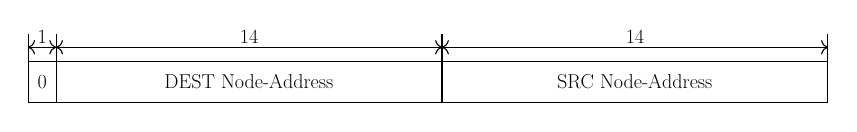
\begin{tikzpicture}[scale=0.35,  every node/.style={scale=0.35},
		region/.style={
			rectangle, 
			minimum height=1.5cm,
			font=\huge}]

		\node (mcast) [region, minimum width=1cm] {0};
		\node (dest) [region, right of=mcast,xshift=6.5cm, minimum width=14cm] {DEST Node-Address};
		\node (src) [region, right of=dest,xshift=13cm, minimum width=14cm] {SRC Node-Address};

		\draw (mcast.north west) -- (src.north east);
		\draw (mcast.south west) -- (src.south east);
		\draw (mcast.south west) -- ++(0,2.5cm);
		\draw (mcast.south east) -- ++(0,2.5cm);
		\draw (dest.south east) -- ++(0,2.5cm);
		\draw (src.south east) -- ++(0,2.5cm);
		\draw[<->] ($(mcast.north west) + (0,0.5cm)$) -- ($(mcast.north east) + (0,0.5cm)$) node[midway, above] {\huge 1};
		\draw[<->] ($(mcast.north east) + (0,0.5cm)$) -- ($(dest.north east) + (0,0.5cm)$) node[midway, above] {\huge 14};
		\draw[<->] ($(dest.north east) + (0,0.5cm)$) -- ($(src.north east) + (0,0.5cm)$) node[midway, above] {\huge 14};
	\end{tikzpicture}
	\caption{Unicast Node-Address to Identifier Mapping}
	\label{fig:des_unicast_addr_to_id}
	\end{center}
\end{figure}

\autoref{fig:des_unicast_addr_to_id} depicts the mapping from source node-address and destination node-address to the CAN identifier for unicast traffic.
The uppermost bit, the multicast bit, is set to zero.
The destination node-address is located in the upper 14 bits, and the source node-address is located in the lower 14 bits.


\subsection{Multicast Address}
\label{sec:multicast_addr}

\begin{figure}[htp]
	\begin{center}
	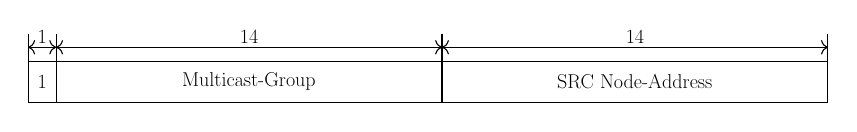
\begin{tikzpicture}[scale=0.35,  every node/.style={scale=0.35},
		region/.style={
			rectangle, 
			minimum height=1.5cm,
			font=\huge}]

		\node (mcast) [region, minimum width=1cm] {1};
		\node (dest) [region, right of=mcast,xshift=6.5cm, minimum width=14cm] {Multicast-Group};
		\node (src) [region, right of=dest,xshift=13cm, minimum width=14cm] {SRC Node-Address};

		\draw (mcast.north west) -- (src.north east);
		\draw (mcast.south west) -- (src.south east);
		\draw (mcast.south west) -- ++(0,2.5cm);
		\draw (mcast.south east) -- ++(0,2.5cm);
		\draw (dest.south east) -- ++(0,2.5cm);
		\draw (src.south east) -- ++(0,2.5cm);
		\draw[<->] ($(mcast.north west) + (0,0.5cm)$) -- ($(mcast.north east) + (0,0.5cm)$) node[midway, above] {\huge 1};
		\draw[<->] ($(mcast.north east) + (0,0.5cm)$) -- ($(dest.north east) + (0,0.5cm)$) node[midway, above] {\huge 14};
		\draw[<->] ($(dest.north east) + (0,0.5cm)$) -- ($(src.north east) + (0,0.5cm)$) node[midway, above] {\huge 14};
	\end{tikzpicture}
	\caption{Multicast-Group to Identifier Mapping}
	\label{fig:des_multicast_to_id}
	\end{center}
\end{figure}

\autoref{fig:des_multicast_to_id} depicts the mapping from source node-address and the multicast group to the CAN identifier for multicast traffic.
The uppermost bit, the multicast bit, is set to one.
The desired multicast group is located in the upper 14 bits, and the source node-address is located in the lower 14 bits.
The multicast group corresponds to the lower 14 bits of the IPv6 multicast address.
As shown in \autoref{sec:ipv6} \autoref{fig:ipv6_multicast_addr}, the Group-ID is located at the lower 112 bits of the IP address.
Using the lower 14 bits is very efficient because all well-known multicast groups fit in that range.
The node can also receive messages with a multicast Group-ID larger than 14 bits,
but these messages may be ambiguous and need to be filtered afterward by the IPv6 address.

\subsection{Address Generation}
\label{sec:address_generation}

Every node is addressed by a 14-bit address as described in \autoref{sec:addressing_schema}.
A node can either have a statically assigned address, or it can pick a random address whenever it connects to the bus or restarts the interface.
In the case of a random address assignment, multiple nodes might attempt to claim the same address at the same time.
Two nodes with the same address would be a violation of the requirement that every node must have a unique address on the bus.
To prevent this situation, \autoref{sec:lldad} describes a mechanism to detect address duplications on the bus.
A node that tries to claim an address already in use can then choose another address and rerun the detection for duplicate addresses.

Random address assignment allows nodes to join the network without any prior knowledge of the other nodes and without being provisioned first.
It is especially useful for nodes that do not have an interface to enter an address or lack of none volatile memory.
The drawback is that the address of a node may change their address whenever it reenters the network.

\subsection{Link-Layer Duplicate Address Detection}
\label{sec:lldad}

To evaluate the need of the Link-Layer duplicate address detection lets first calculate the probability that two devices choose the same address,
when they use an independent random number to assign their address.
The address space a node can take its address from is 0x0100 to 0x3DEF (15599).
Let us assume that we have 100 nodes on the bus.
Depending on the transceivers used and wiring, this is a realistic electrical limit.

Let $N$ be the number of possible addresses, $n$ the number of nodes, and $P$ the probability for a collision. 
The number of possible permutations of addresses and nodes is $N^n = 15599^{100}$.\\
The number of permutations without a collision is \\ $N \cdot (N-1) \cdot ... \cdot (N - (n - 1))$.\\
Using the Laplace formula gives \autoref{eq:prop_col}.

\begin{equation}
	\begin{split}
		P = 1 - \frac{N \cdot (N-1) \cdot ... \cdot (N - (n - 1))}{N^n} \\
		P = 1 - \frac{\displaystyle\prod_{i=1}^{n} N - (i - 1)}{N^n} = 1 -\frac{n! \cdot \binom{N}{n}} {N^n}
	\end{split}
	\label{eq:prop_col}
	\end{equation}
	
	\begin{equation}
		P = 1 - \frac{100! \cdot \binom{15599}{100}}{15599^{100}} \approx 0.2724
	\label{eq:prop_col_res}
	\end{equation}

\autoref{eq:prop_col_res} is the result of our example with 100 nodes.

The probability of having a collision is therefor 27.24\%.
For most applications, this number unacceptable, and a mechanism to prevent collisions needs to be applied.

For this reason, we introduced the Link-Layer duplicate address detection (LLDAD).
LLDAD works on the Link-Layer only and utilizes a special CAN frame type, the Remote Transmission Request (RTR).

\input{figures/des_dad_request}

The collision detection begins with sending an LLDAD-request.
The LLDAD-request is an RTR frame with no data.
The 29-bit identifier has the same address-layout as a unicast 6LoCAN frame, but the source address is filled with entropy,
and the destination address is filled with the tentative address as shown in  \autoref{fig:des_lldad_req}.
The entropy prevents collisions in case another node tries to acquire the same address at the same time.
The probability of not having a collision with 100 nodes, performing LLDAD at the same time, is calculated in \autoref{eq:prop_col_dad}.
The equation uses a slightly modified formula from \autoref{eq:prop_col} with an address range extended by the 14-bit entropy.

\begin{equation}
	P = \frac{100! \cdot \binom{15599 \cdot 2^{14}}{100}}{(15599 \cdot 2^{14})^{100}} \approx 0.99998
\label{eq:prop_col_dad}
\end{equation}

\input{figures/des_dad_response}

After the LLDAD-request is sent, the node waits at least 100ms for an LLDAD response frame.
The response-frame is not an RTR frame and does not contain data.
The identifier of the response is shown in \autoref{fig:des_lldad_resp}.
The destination-address is the LLDAD response address 0x3DFE, and the source address is the address of the node that already owns the address,
which is the same address as the tentative address.
If there is no LLDAD-response frame with the tentative address as the source address on the bus,
the tentative address is considered to be unique and becomes the address of the node.
If the node receives an LLDAD-response, the LLDAD is failed, and in case the address was randomly chosen, it can retry with another random address.
If the address was statically assigned, the node is not allowed to use the address and, therefore, cannot bring up the interface.

\begin{figure}[htp]
	\begin{center}
	\begin{tikzpicture}[scale=0.6, node distance=2cm, every node/.append style={scale=0.6}]
		\node (start) [startstop] {Interface Up};
		\node (ll_ten) [process, below = of start] {Chose Tentative Link-Local Address (static address or random)};
		\node (lldad_req) [io, below = of ll_ten] {Send LLDAD-Request};
		\node (lldad_resp) [io, below = of lldad_req] {Wait for LLDAD-Response or 100ms Timeout};
		\node (lldad) [decision, below = of lldad_resp] {LLDAD-Response received?};
		\node (rand) [decision, right of=lldad, xshift=7cm] {Random address?};
		\node (lldad_fail) [startstop, below = of rand] {LLDAD failed};
		\node (success) [startstop, below = of lldad] {Use Tentative Address as Node Address};

		\draw [arrow] (start) -- (ll_ten);
		\draw [arrow] (ll_ten) -- (lldad_req);
		\draw [arrow] (lldad_req) -- (lldad_resp);
		\draw [arrow] (lldad_resp) -- (lldad);
		\draw [arrow] (lldad) -- node [anchor=south] {yes (LLDAD failed)} (rand);
		\draw [arrow] (lldad) -- node [anchor=east] {no (LLDAD succeeded)} (success);
		\draw [arrow] (rand) |- node [anchor=south] {yes} (ll_ten);
		\draw [arrow] (rand) -- node [anchor=east] {no} (lldad_fail);
	\end{tikzpicture}
	\end{center}
	\caption{Link-Layer Duplicate Address Detection}
	\label{fig:des_lldad}
\end{figure}

\autoref{fig:des_lldad} depicts the procedure of the LLDAD.

\section{Stateless Address Autoconfiguration}
\label{sec:impl_slaac}

The process of creating an IPv6 address is defined in \autoref{sec:ipv6_slaac}.
However, forming the interface identifier depends on the underlying Link-Layer.
The process of creating an interface identifier does not strictly follow the rules of RFC4291 \cite{rfc4291} Appendix A.
Instead of taking the 14-bit node address and zero fill it to the left, we use the method of creating an identifier from a 48-bit identifier.
The reason for this is that this method was also chosen for 6LoWPAN (RFC4944 \cite{rfc4944}) and the header compression
is most efficient when the interface identifier if formed in that way.

For example, a node with the node-address of 0x1234 would create the interface identifier ::ff:fe00:1234/64.

Since the node address is only guaranteed to be unique on the bus-segment, the IPv6 Duplicate Address detection,
as described in \autoref{sec:ipv6_slaac}, needs to be performed.
If the DAD failed, the node can either pick a new node-address or form an interface identifier that is not related to the node-address.
The latter would result in an inefficient header compression and should, therefore, be avoided.

\section{ISO-TP for 6LoCAN}
\label{sec:iso_tp_6LoCAN}

IPv6 defines that the minimal MTU is 1280 bytes, but a CAN frame has a payload length of eight bytes for classical CAN and 64 bytes for CAN-FD.
To satisfy the minimal MTU requirement, 6LoCAN uses a slightly modified version of ISO-TP.
Some features like the address extension are not useful and, therefore, not used and not supported.
The maximum packet size is limited to 4095 bytes, to limit the PCI of the first frame to two bytes.
TSO-TP does only support unicast data transfer, but for IPv6, it is necessary to have multicast traffic too.
Hence, we defined a way to have multicast transmissions, but without flow control.

\subsection{Multicast}
\label{sec:multicast_iso_tp}

For multicast packets, we cannot have flow control, because there is more than one node receiving the packet and therefore,
more than one node that would answer with a flow control frame.
The sender cannot handle flow control for more than one receiving node because he does not know who and how many receivers there are.

\begin{figure}[htp]
\begin{center}
	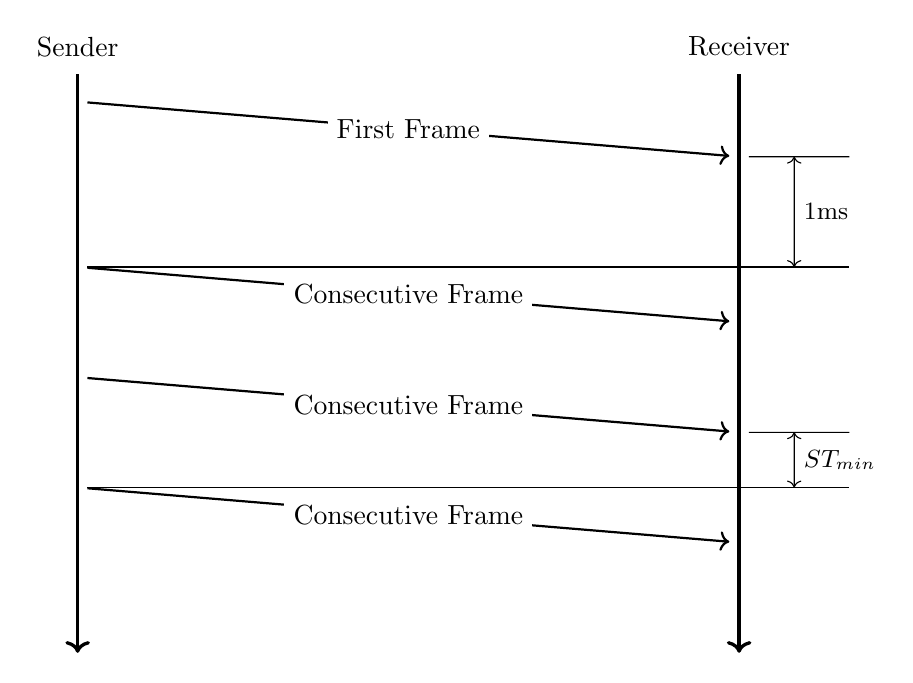
\begin{tikzpicture}[scale=0.7]
		%Sender
		\node (s_ff) at (0,10)  {};
		\node (s_cf1) at (0,7) {};
		\node (s_cf2) at (0,5) {};
		\node (s_cf3) at (0,3) {};
		
		%Receiver
		\node (r_ff) at (12,9)  {};
		\node (r_cf1) at (12,6) {};
		\node (r_cf2) at (12,4) {};
		\node (r_cf3) at (12,2) {};


		%connections
		\draw[thick, ->] (s_ff) -- node[midway, fill=white] {First Frame} (r_ff);
		\draw[thick,->] (s_cf1) -- node[midway, fill=white] {Consecutive Frame} (r_cf1);
		\draw[thick,->] (s_cf2) -- node[midway, fill=white] {Consecutive Frame} (r_cf2);
		\draw[thick,->] (s_cf3) -- node[midway, fill=white] {Consecutive Frame} (r_cf3);
		
		%FF - CF time
		\draw (r_ff) -- ++(2,0);
		\draw (s_cf1) -- ++(14,0);
		\draw[<->] ($(r_ff) + (1,0)$) -- ($(s_cf1) + (13,0)$) node[midway,right]{\small 1ms};

		%stmin
		\draw (r_cf2) -- ++(2,0);
		\draw (s_cf3) -- ++(14,0);
		\draw[<->] ($(r_cf2) + (1,0)$) -- ($(s_cf3) + (13,0)$) node[midway,right]{\small $ST_{min}$};
		
		%Flow
		\draw[very thick, ->] (0,10.5) --  (0,0);
		\node at (0,11) {Sender};
		\draw[very thick, ->] (12,10.5) -- (12,0);
		\node at (12,11) {Receiver};
		
	\end{tikzpicture}
	\caption{Example Multicast Sequence}
	\label{fig:des_iso_tp_mcast}
\end{center}
\end{figure}

\autoref{fig:des_iso_tp_mcast} shows the sequence of a multicast transfer.
6LoCAN defines that there has to be a pause between the First Frame and the first Consecutive Frame of at least 1ms.
This pause allows all receiving nodes to set-up the CAN filter and allocate memory for the reception of the frame.
The $ST_{min}$ has to be chosen such that the slowest node on the bus can handle the reception.
Multicast traffic is slower and maybe more unreliable than unicast transfers.
For packets that fit in a Single Frame packet, multicast works the same way as unicast does.

\subsection{Ethernet Border Translator}
\label{sec:eth_border_translator}

\input{figures/des_bordertrans}

The Ethernet Border Translator is a concept for connecting a 6LoCAN bus segment to an Ethernet network.
It is neither a router nor a switch.
It only translates the packets from one Link-Layer to another, which means that the nodes stay in the same Link-Local domain.
The advantage of this concept is that the translator is fully stateless and does not need any configuration and knowledge of the network.
It allows us to use small devices with very little memory to be used as Border Translators.
In case the 6LoCAN network segment needs a router, the Border Translator can be used to connect the 6LoCAN network to an ordinary Ethernet router.
The Ethernet Border Translator can also be used to connect multiple 6LoCAN bus segments, using a standard Ethernet Switch.
With the Ethernet Border Translator, we can use already existing Ethernet equipment for routing 6LoCAN traffic in the network.
The advantage of keeping the devices in the same Link-Local domain is that multicast discovery protocols still works.

The translator has a fixed CAN node address (0x3DF0).
With having a fixed address for the translator, the other nodes do not need a mechanism for discovering translators.
6LoCAN nodes do not need to know if a destination node the want to reach is in the same network, or connected via a translator.
The sending node only needs to perform a neighborhood discovery as described in \autoref{sec:ipv6_ndp}.
The border translator then forwards the neighbor solicitation message, and if the node is behind the translator,
the answer will be forwarded by the translator.
Since the address of the translator is well known, a node automatically knows that the packet is from outside the CAN bus segment,
if the source node-address is the translator address.
Packets forwarded from Ethernet to 6LoCAN carry the original 48 bit Ethernet MAC address directly after the ISO-TP First Frame header.
Since the First Frame header has a size of two bytes, the inlined address always fits in the remaining frame data.
A node receiving a packet from the border translator now replaces the node-address with the in-lined MAC address and saves it to the neighborhood cache.
The node can now decide from the size of the address, stored in the neighborhood cache,
if the packets need to be sent to the translator or to a node within the same bus-segment.
Packets originating from a 6LoCAN node with a destination behind the translator are sent to the node-address of the translator
and carry the destination Ethernet MAC-address inline.
The border translator reassembles the packet, uncompresses the IPv6 header, and forwards the packet to the destination MAC-address.
The source MAC-address is the 14-bit 6loCAN node-address extended by a 34-bit prefix.
For packets from Ethernet to 6LoCAN, the translator compresses the IPv6 header and performs an ISO-TP transmission to the destination node.
The destination node-address is taken from the last 14 bits of the destination MAC-address.

For neighborhood discovery packets, originating from the 6LoCAN network, with a Link-Layer address option (see \autoref{sec:ipv6_ndp}),
the translator has to inspect the packet and extend the address in the option to match the extended Ethernet MAC-address.

\begin{figure}[htp]
	\begin{center}
	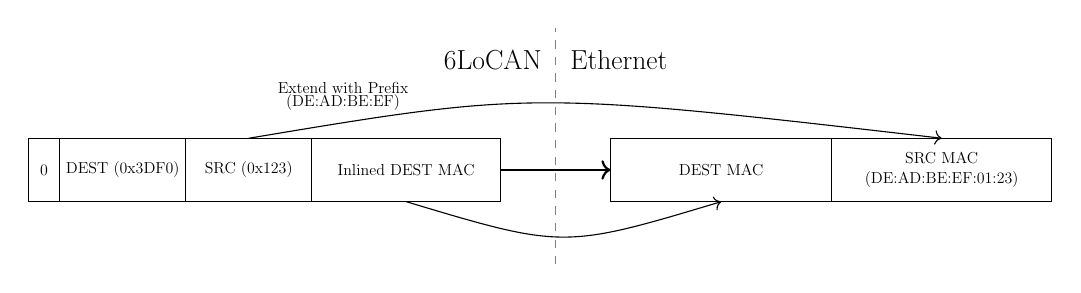
\begin{tikzpicture}[scale=0.4,  every node/.style={scale=0.4},
		region/.style={
			rectangle,
			draw,
			align=center,
			font=\Large,
			minimum height=2cm}]

		\node (mcast) [region, minimum width=1cm] {0};
		\node (dest) [region, right of=mcast,xshift=1.5cm, minimum width=4cm] { DEST (0x3DF0)};
		\node (src) [region, right of=dest,xshift=3cm, minimum width=4cm] {SRC (0x123)};
		\node (dstmacil) [region, right of=src,xshift=4cm, minimum width=6cm] {Inlined DEST MAC};

		\node (dstmac) [region, right of=dstmacil, xshift=9cm, minimum width=7cm] {DEST MAC};
		\node (srcmac) [region, right of=dstmac, xshift=6cm, minimum width=7cm] {SRC MAC \\ (DE:AD:BE:EF:01:23)};

		\draw[thick, ->] (dstmacil.east) -- (dstmac.west) coordinate[midway](border);
		\draw[dashed, black!50] ($(border) + (0,-3cm)$) -- ($(border) + (0,4.5cm)$);
		\node at ($(border) + (-2cm,3.5cm)$) {\Huge 6LoCAN};
		\node at ($(border) + (2cm,3.5cm)$) {\Huge Ethernet};
		\draw[->] (dstmacil.south) .. controls ++(5cm,-1.5cm) .. (dstmac.south);
		\draw[->] (src.north) .. controls ++(9cm,1.5cm) .. (srcmac.north) node [align=center, very near start, above, yshift=0.25cm] {\Large Extend with Prefix \\ \Large(DE:AD:BE:EF)};
	\end{tikzpicture}
	\caption{6LoCAN to Ethernet Address Translation}
	\label{fig:bordertrans_6lo_eth}
	\end{center}
\end{figure}
\begin{figure}[htp]
	\begin{center}
	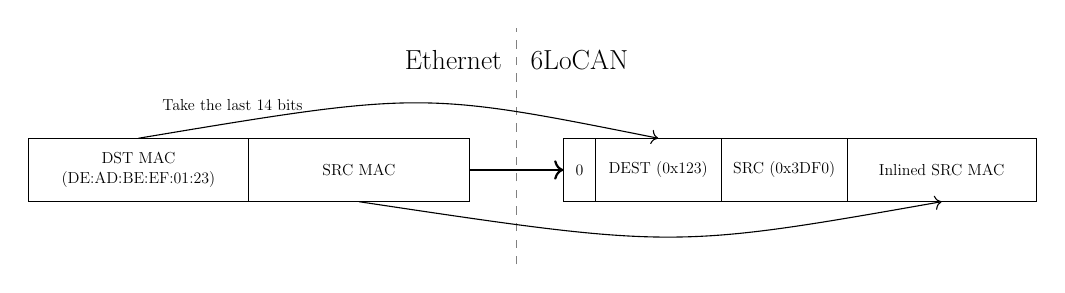
\begin{tikzpicture}[scale=0.4,  every node/.style={scale=0.4},
		region/.style={
			rectangle,
			draw,
			font=\Large,
			align=center,
			minimum height=2cm}]

		\node (dstmac) [region,, minimum width=7cm] {DST MAC \\ (DE:AD:BE:EF:01:23)};
		\node (srcmac) [region, right of=dstmac, xshift=6cm, minimum width=7cm] {SRC MAC};

		\node (mcast) [region,right of=srcmac, xshift=6cm, minimum width=1cm] {0};
		\node (dest) [region, right of=mcast,xshift=1.5cm, minimum width=4cm] {DEST (0x123)};
		\node (src) [region, right of=dest,xshift=3cm, minimum width=4cm] {SRC (0x3DF0)};
		\node (dstmacil) [region, right of=src,xshift=4cm, minimum width=6cm] {Inlined SRC MAC};

		\draw[thick, ->] (srcmac.east) -- (mcast.west) coordinate[midway](border);
		\draw[dashed, black!50] ($(border) + (0,-3cm)$) -- ($(border) + (0,4.5cm)$);
		\node at ($(border) + (-2cm,3.5cm)$) {\Huge Ethernet};
		\node at ($(border) + (2cm,3.5cm)$) {\Huge 6LoCAN};
		\draw[->] (srcmac.south) .. controls ++(10cm,-1.5cm) .. (dstmacil.south);
		\draw[->] (dstmac.north) .. controls ++(9cm,1.5cm) .. (dest.north) node [align=center, very near start, above, yshift=0.25cm]{\Large Take the last 14 bits};
	\end{tikzpicture}
	\caption{Ethernet to 6LoCAN Address Translation}
	\label{fig:bordertrans_eth_6lo}
	\end{center}
\end{figure}

\autoref{fig:bordertrans_6lo_eth} shows how the 6LoCAN node address is extended to an Ethernet MAC-address and 
\autoref{fig:bordertrans_eth_6lo} shows how the Ethernet MAC-address address is extended to a 6LoCAN node address.

\chapter{Implementation}
\label{cha:implementation}

The 6LoCAN protocol is implemented into the Zephyr RTOS and made its way to the 2.0 release.
The implementation was made in two phases.
First we introduced a generic CAN API and an implementation of it for the STM32 microcontroller platform.
In the second phase, I implemented the 6LoCAN translation layer into the Zephyr networking stack.

\section{The Zephyr CAN API}
\label{sec:can_api}
Before this work, the Zephyr RTOS was lacking a CAN API, so the first step was to create a platform-agnostic API.
The API should only support features defined by the CAN specification \cite{BoschCAN},
to ensure that the network or application layer can rely on the API features.

The first API had an interface for the following features:
\begin{itemize}
        \item Configure the mode and bitrate of the controller.
        \item Send a frame
        \item Attach a CAN filter and submit a callback whenever the filter matches on a frame
        \item Attach a CAN filter and submit the frame to a message queue whenever the filter matches
        \item Detach attached filters
\end{itemize}

It also defined containers for CAN frames and CAN filters called zcan\_frame and zcan\_filter.
The containers provide a platform-agnostic way to handle frames and filters.
The specific driver implementation is responsible for converting the zcan\_frame and zcan\_filter to the respective register values.

The Zephyr community agreed on my API proposal and the implementation for the STM32 platform and it was merged merged into Zephyr version 1.12.
The API evolved over the time and got extended by an API the get the bus state and recover from bus-off state.
Additionally people from the Zephyr community added two other driver implementations.
One for an external CAN controller (MCP2515) and one for NXP platforms, based on NXPs flexcan IP.

\subsection{Zephyr CAN frame}
\begin{lstlisting}[style=ccode, numbers=none]
struct zcan_frame {
	u32_t id_type : 1;
	u32_t rtr     : 1;
	u32_t ext_id  : 29;
	u8_t  dlc;
	u8_t  data[8];
};
\end{lstlisting}
The struct above shows a simplified version of a Zephyr CAN frame.
It is a container for a CAN frame and includes the identifier type, the identifier, a flag for RTR frames, the data length code, and the data data.

\subsection{Zephyr CAN filter}
\begin{lstlisting}[style=ccode, numbers=none]
struct zcan_filter {
	u32_t id_type  : 1;
	u32_t rtr      : 1;
	u32_t ext_id   : 29;

	u32_t rtr_mask    : 1;
	u32_t ext_id_mask : 29;
}
\end{lstlisting}
The struct above shows a simplified version of a Zephyr CAN filter struct.
It is a container for a CAN filter and includes the identifier type, the identifier, the RTR bit, and the masks for the identifier and RTR-bit.
The mask signals which bits of the identifier should be taken into account during the filtering.
Bits that are set to one are compared and bits that are zero are ignored.
Lets take an example of a filter with an identifier of 0x123 and a mask of 0xff.
Frames with the identifier 0x123, 0x223, or generally 0xX23, where X is any number, would pass the filter.
Frames with the identifier 0x124, 0x133, or generally 0xYXX, where XX is not 0x23, will not pass the filter.

\subsection{Sending CAN frames}
\begin{lstlisting}[style=ccode, numbers=none]
int can_send(struct device *dev, const struct zcan_frame *msg,
             s32_t timeout, can_tx_callback_t callback_isr,
             void *callback_arg);
\end{lstlisting}
The Send API is defined as shown above.
It takes a pointer to the CAN device, a pointer to the frame container, a timeout, a callback function and an argument that is passed to the callback function.
The function sends the frame as soon as a mailbox is ready to send a message.
If a NULL pointer is passed to as the callback function, the call blocks until the message is sent.
Otherwise the callback is called when the message is sent.

\subsection{Receiving CAN frames}

\begin{lstlisting}[style=ccode, numbers=none]
int can_attach_isr(struct device *dev,
                   can_rx_callback_t isr, void *callback_arg,
                   const struct zcan_filter *filter);
\end{lstlisting}
The main receiving function is shown above.
It takes a pointer to the CAN device, the function that should be called when a frame that passes the filter is received,
an argument that is passed to the callback and the CAN filter.
The function returns a filter-id to uniquely identify the attached filter.
The filter-id is used for detaching the filter when needed.
The CAN controller reads any message on the bus and compares the identifier to the attached filters.
If a filter matches, the respective callback is called.
If the identifier matches more that one filter, the function called depends on the metrics of the CAN controller.
The callback is called in an interrupt context and therefor is not allowed to block and should keep the execution time as low as possible.

\begin{lstlisting}[style=ccode, numbers=none]
int can_attach_workq(struct device *dev, struct k_work_q *work_q,
                     struct zcan_work *work,
                     can_rx_callback_t callback,
                     void *callback_arg,
                     const struct zcan_filter *filter);
\end{lstlisting}
The can\_attach\_workq function is a wrapper for the can\_attach\_isr,
that calls the callback function in the context of the provided work queue instead of an ISR context.

\begin{lstlisting}[style=ccode, numbers=none]
int can_attach_msgq(struct device *dev, struct k_msgq *msg_q,
                    const struct zcan_filter *filter);
\end{lstlisting}
The can\_attach\_msgq function attaches a message queue instead on a callback.
Whenever a frame that matches the filter is received, it is put into the message queue.
The message queue can then be read within a thread.

\section{6LoCAN Implementation}
\label{sec:6locan_impl}

\begin{figure}[htp]
	\begin{center}
	\begin{tikzpicture}[
		scale=0.7,
		every node/.append style={scale=0.7},
		layers/.style={
			align=left,
			fill=blue!5,
			rectangle,
			draw=blue!5,
			minimum width = 12cm,
			node distance=0.2cm},
		layers_dark/.style={
			draw=black,
			fill=blue!15,
			rectangle,
			minimum width = 12cm,
			minimum height = 1cm,
			node distance=0.2cm},
		layer_rot/.style={
			draw=black,
			fill=blue!15,
			rectangle},
		instance/.style={
			draw=black,
			rounded corners=0.05cm,
			fill=blue!15,
			rectangle, 
			minimum width=2cm,
			minimum height=1cm,
			align=center,
			font=\small},
		instance_wide/.style={
			draw=black,
			rounded corners=0.05cm,
			fill=blue!15,
			rectangle, 
			minimum width=4cm,
			minimum height=1cm,
			align=center,
			font=\small}
		]

		%App
		\node (app)[layers_dark] {Networking Application};
	
	
	
		%Sockets API
		\node (sockets)[layers_dark, below = of app.south west,anchor=north west] {Sockets API};

		%Net-context
		\node (netctx)[layers_dark, below = of sockets.south west,anchor=north west] {Net-Context API};
	
		%Transport-Layer Protocols
		\node (transp)[layers,below = of netctx.south west,anchor=north west, text width = 9.1cm, minimum height = 4cm, text depth = 3cm] {Transport-Layer Protocols};
		\foreach \tansport/\x/\y in {ICMPv4/-2.5/0.75, ICMPv6/2.5/0.75, TCP/-2.5/-0.5, UDP/2.5/-0.5}{
			\node (\tansport) at ($(transp) + (\x cm, \y cm -0.5 cm)$) [instance_wide] {\tansport};
		}

		%Networking Protocols
		\node (netw)[layers,below = of transp.south west,anchor=north west, text width=9.1cm, minimum height = 2.5cm, text depth = 1.5cm] {Networking Protocols};
		\foreach \network/\x in {IPv4/-2.5, IPv6/2.5}{
			\node (\network) at ($(netw) + (\x cm, -0.5 cm)$) [instance_wide] {\network};
		}

		%Interface Abstraction
		\node (netcore)[layers_dark, below = of netw.south west,anchor=north west] {Network Core};

		%Interface Abstraction
		\node (interf)[layers_dark, below = of netcore.south west,anchor=north west] {Network Interface Abstraction Layer};

		%Link-Layer
		\node (linklayer)[layers, below = of interf.south west,anchor=north west, text width = 10.3cm, minimum height = 2.5cm, text depth = 1.5cm] {Link-Layer Technologies};
		\foreach \linklayer/\x/\col in {Ethernet/-4/blue!15, 6LoWPAN/-1.25/blue!15, 6LoCAN/1.25/green!15, IPSP/4/blue!15}{
			\node (\linklayer) at ($(linklayer) + (\x cm, -0.5 cm)$) [instance, fill=\col] {\linklayer};
		}

		%Network drivers
		\node (net_drivers)[layers, below = of linklayer.south west,anchor=north west, text width = 11.5cm, minimum height = 3cm, text depth = 2cm] {Network Device Drivers};
		\foreach \driver/\x/\col in {Ethernet/-4.5/blue!15, CAN/-1.5/green!15, 802.15.4/1.5/blue!15, Other/4.5/blue!15}{
			\foreach \inst in {0.3,0.2,0.1}{
				\node at ($(net_drivers) + (\x cm - \inst cm, -0.5 cm + \inst cm)$) [instance] {};
			}
			\node (\driver)  at ($(net_drivers) + (\x cm, -0.5 cm)$) [instance, fill=\col] {\driver \\ drivers};
		}

		\draw [arrow] (CAN.north) -- node[yshift=-1.5cm,draw, circle, anchor=west, xshift=0.1cm]{1} (netcore.south -| CAN.north);
		\draw [arrow] ([xshift=1cm]netcore.south) coordinate (netcore1) -- node[draw, circle, anchor=east, xshift=-0.1cm]{2} (interf.north -| netcore1);
		\draw [arrow_rev] ([xshift=1.5cm]netcore.south) coordinate (netcore2) -- node[draw, circle, anchor=west, xshift=0.1cm]{5} (interf.north -| netcore2);
		\draw [arrow_rev] ([xshift=-0.25cm]6LoCAN.north) coordinate (6locan1) --  node[draw, circle, anchor=east, xshift=-0.1cm]{3} (interf.south -| 6locan1);
		\draw [arrow] ([xshift= 0.25cm]6LoCAN.north) coordinate (6locan2) -- node[draw, circle, anchor=west, xshift=0.1cm] {4} (interf.south -| 6locan2);
		\draw [arrow_rev] (IPv6.south) -- node[draw, circle, anchor=west, xshift=0.1cm] {6} (netcore.north -| IPv6.south);
		\draw [arrow] ([xshift=0.25cm]IPv6.north) coordinate (udp1) -- node[draw, circle, anchor=west, xshift=0.1cm] {7} (UDP.south -| udp1);
		\draw [arrow_rev] ([xshift=-0.25cm]IPv6.north) coordinate (udp2) -- node[draw, circle, anchor=east, xshift=-0.1cm] {8} (UDP.south -| udp2);
		\draw [arrow] ([xshift=-1cm]IPv6.north) -- node[draw, circle, anchor=east, xshift=-0.1cm, yshift=-0.1cm] {9} (netctx);
		\draw [arrow] (netctx) -- node[draw, circle, anchor=east, xshift=-0.1cm] {10} (sockets);
		\draw [arrow] (sockets.north) -- node[draw, circle, anchor=east, xshift=-0.1cm] {11} (app.south);
	\end{tikzpicture}
	\caption{Zephyr Network Stack 6LoCAN RX example}
	\label{fig:zephyr_net_stack_rx}
	\end{center}
\end{figure}


A Link-Layer Implementation in Zephyr consist of two layers.
The Network Device Driver and the Link-Layer implementation (L2), which are highlighted in \autoref{fig:zephyr_net_stack_rx}.
For the 6LoCAN implementation, the Network Device Driver is an abstraction of the Zephyr CAN API that installs the respective frame filters,
handles the incoming CAN frames in an interrupt context, puts them into network packets, sets the Link-Layer address of them,
and and hands the packet over to the receiving work-queue. For sending CAN frames, the abstraction only forwards the raw CAN frames.
The 6LoCAN Link-Layer implementation does the parsing of the ISO-TP header, fragmentation and reassembly, and IPHC header compression and decompression.
The device driver implementation is explained in detail in \autoref{sec:6locan_net_dev},
and the L2 implementation is explained in detail in \autoref{sec:6locan_l2}.

\newpage

\autoref{fig:zephyr_net_stack_rx} shows an example of receiving a UDP packet.
\begin{enumerate}
        \item The CAN network device driver uses the CAN API to receive the raw CAN frames.
              The frames are copied into network packets and handed over to the Net Core.
              The Net Core accepts the packet and puts it into a receiving work-queue, depending on the priority of the packet.
        \item When the receiving queue is scheduled, the packet is handed over to the Network Interface.
        \item The Network Interface calls the 6LoCAN L2 implementation with the received packet, which analyzes the frame content.
              The L2 implementation performs the reassembly (ISO-TP) and when the packet is complete, the IPHC decompression.
        \item If the packet is complete and decompression is successful, the reassembled packet is passed back to the Network Interface.
        \item The packet is then forwarded to the Net Core.
        \item The Network Core checks the IP header version and if it is IPv6, the IPv6 implementation is called.
              The IPv6 implementation checks the IPv6 headers and discards the packet if the destination does not match any addresses of the interface.
        \item Depending on the next header field, the specific transport layer implementation is called. In this Example, it is UDP.
        \item The UDP implementation parses the UDP header, checks the checksum and length of the packet, and returns the result to the IPv6 implementation.
        \item If the packet is valid, the IPv6 implementation passes the packet to the Net-Context API.
        \item The Net-Context API checks for registered sockets on the destination-port.
        \item If a socket is listening to the destination-port, the Socket-API passes the packet to the networking-application.
\end{enumerate}

\newpage
\begin{figure}[htp]
	\begin{center}
	\begin{tikzpicture}[
		scale=0.7,
		every node/.append style={scale=0.7},
		layers/.style={
			align=left,
			fill=blue!5,
			rectangle,
			draw=blue!5,
			minimum width = 12cm,
			node distance=0.2cm},
		layers_dark/.style={
			draw=black,
			fill=blue!15,
			rectangle,
			minimum width = 12cm,
			minimum height = 1cm,
			node distance=0.2cm},
		layer_rot/.style={
			draw=black,
			fill=blue!15,
			rectangle},
		instance/.style={
			draw=black,
			rounded corners=0.05cm,
			fill=blue!15,
			rectangle, 
			minimum width=2cm,
			minimum height=1cm,
			align=center,
			font=\small},
		instance_wide/.style={
			draw=black,
			rounded corners=0.05cm,
			fill=blue!15,
			rectangle, 
			minimum width=4cm,
			minimum height=1cm,
			align=center,
			font=\small}
		]

		%App
		\node (app)[layers_dark] {Networking Application};
	
	
	
		%Sockets API
		\node (sockets)[layers_dark, below = of app.south west,anchor=north west] {Sockets API};

		%Net-context
		\node (netctx)[layers_dark, below = of sockets.south west,anchor=north west] {Net-Context API};
	
		%Transport-Layer Protocols
		\node (transp)[layers,below = of netctx.south west,anchor=north west, text width = 9.1cm, minimum height = 4cm, text depth = 3cm] {Transport-Layer Protocols};
		\foreach \tansport/\x/\y in {ICMPv4/-2.5/0.75, ICMPv6/2.5/0.75, TCP/-2.5/-0.5, UDP/2.5/-0.5}{
			\node (\tansport) at ($(transp) + (\x cm, \y cm -0.5 cm)$) [instance_wide] {\tansport};
		}

		%Networking Protocols
		\node (netw)[layers,below = of transp.south west,anchor=north west, text width=9.1cm, minimum height = 2.5cm, text depth = 1.5cm] {Networking Protocols};
		\foreach \network/\x in {IPv4/-2.5, IPv6/2.5}{
			\node (\network) at ($(netw) + (\x cm, -0.5 cm)$) [instance_wide] {\network};
		}

		%Interface Abstraction
		\node (netcore)[layers_dark, below = of netw.south west,anchor=north west] {Network Core};

		%Interface Abstraction
		\node (interf)[layers_dark, below = of netcore.south west,anchor=north west] {Network Interface Abstraction Layer};

		%Link-Layer
		\node (linklayer)[layers, below = of interf.south west,anchor=north west, text width = 10.3cm, minimum height = 2.5cm, text depth = 1.5cm] {Link-Layer Technologies};
		\foreach \linklayer/\x/\col in {Ethernet/-4/blue!15, 6LoWPAN/-1.25/blue!15, 6LoCAN/1.25/green!15, IPSP/4/blue!15}{
			\node (\linklayer) at ($(linklayer) + (\x cm, -0.5 cm)$) [instance, fill=\col] {\linklayer};
		}

		%Network drivers
		\node (net_drivers)[layers, below = of linklayer.south west,anchor=north west, text width = 11.5cm, minimum height = 3cm, text depth = 2cm] {Network Device Drivers};
		\foreach \driver/\x/\col in {Ethernet/-4.5/blue!15, CAN/-1.5/green!15, 802.15.4/1.5/blue!15, Other/4.5/blue!15}{
			\foreach \inst in {0.3,0.2,0.1}{
				\node at ($(net_drivers) + (\x cm - \inst cm, -0.5 cm + \inst cm)$) [instance] {};
			}
			\node (\driver)  at ($(net_drivers) + (\x cm, -0.5 cm)$) [instance, fill=\col] {\driver \\ drivers};
		}

		\draw [arrow] (app.south) -- node[draw, circle, anchor=east, xshift=-0.1cm] {1} (sockets.north);
		\draw [arrow] (sockets) -- node[draw, circle, anchor=east, xshift=-0.1cm] {2} (netctx);
		\draw [arrow_both] ([xshift=0.5cm]IPv6.north) coordinate (IPv61) -- node[draw, circle, anchor=west, xshift=0.1cm, yshift=2cm] {3} (netctx.south -| IPv61);
		\draw [arrow_both] ([xshift=-0.5cm]UDP.north) coordinate (UDP1) -- node[draw, circle, anchor=east, xshift=-0.1cm, yshift=0.5cm] {4} (netctx.south -| UDP1);
		\draw [arrow] (netctx) -- node[draw, circle, anchor=east, xshift=-0.1cm, yshift=-0.5cm] {5} (netcore);
		\draw [arrow] (netcore) -- node[draw, circle, anchor=east, xshift=-0.1cm] {6} (interf);
		\draw [arrow_rev] (6LoCAN.north) coordinate (6locan1) --  node[draw, circle, anchor=east, xshift=-0.1cm]{7} (interf.south -| 6locan1);
		\draw [arrow] (6LoCAN.south) --  node[draw, circle, anchor=east, xshift=-0.1cm, yshift=0.1cm]{8} (CAN.north);

	\end{tikzpicture}
	\caption{Zephyr Network Stack 6LoCAN TX example}
	\label{fig:zephyr_net_stack_tx}
	\end{center}
\end{figure}


\autoref{fig:zephyr_net_stack_tx} shows an example of sending a UDP packet.
\begin{enumerate}
        \item The Application sends a chunk of data by using the Socket-API.
        \item The Socket-API binds the request to the context of the opened socket and uses the API to send the data.
        \item The Net-Context implementation calls the IPv6 implementation to fill the IPv6 headers. The interface information, like the source IP address,
              is taken from the interface associated to the Net-Context.
        \item The Net-Context implementation calls the UDP implementation to fill the UDP headers.
        \item The packet is then handed over to the network core.
        \item The network core calls the Network Interface abstraction, which fills the Link-Layer addresses (from either neighborhood discovery or cache).
        \item The Network Interface abstraction then puts the packet into the sending work-queue. The work-queue thread then calls th 6LoCAN Link-Layer.
              The Link-Layer creates a ISO-TP context and performs the fragmentation.
        \item For every frame that is sent, the CAN network driver is called.
\end{enumerate}

\FloatBarrier
\subsection{6LoCAN Network Device Driver}
\label{sec:6locan_net_dev}

The 6LoCAN Network Device Driver is responsible for receiving and sending RAW CAN frames.
For this purpose it is using the Zephyr CAN API.
The API exposes five functions:
\begin{itemize}
        \item Interface Initialization
        \item Enabling/Disabling
        \item Sending
        \item Attaching Filters
        \item Detaching Filters
\end{itemize}

\textbf{Interface Initialization} binds the driver context to an interface, calls the initialization function of the 6LoCAN Link-Layer and registers the multicast monitor.
The multicast monitor is called whenever a multicast group is added to an interface.

\textbf{Enable} is called from the 6LoCAN Link-Layer whenever the interface changes its state from up (enabled) to down (disabled) or vice versa.
If the interface is going to be brought up, then this function attaches the unicast CAN filter.
This filter receives unicast frames where the destination address matches the interface link-local address.
If the interface is going to be brought to the down state, the unicast filter is detached.

\textbf{Send} forwards the incoming frames to the Zephyr CAN API without any modification.

\textbf{Attach Filter} and \textbf{Detach Filter} are wrappers for the Zephyr CAN API, and work the same way the Zephyr CAN API do.
They are used to attach filters for the Link-Layer Duplicate Address Detection (LLDAD), from the 6LoCAN Link-Layer.

Whenever a frame on the bus matches the unicast filter, the receiving function is called.
This function allocates a net packet that is large enough to hold the frame payload, the source and the destination Link-Layer address.
The addresses are taken from the frame identifier and copied into the packet, followed by the frame payload.
The resulting packet is then put into the receiving work-queue of the network stack, which later passes it to the 6LoCAN Link-Layer.

The multicast monitor is responsible for attaching filters for the corresponding multicast group.
The filter matches the the last 14 bits of the IP address and the multicast flag. The source address is ignored for the comparison.
For receiving the frames, the same receiving function is used, as it is used for unicast frames.

\subsection{6LoCAN Link-Layer}
\label{sec:6locan_l2}

The 6LoCAN Link-Layer gets the raw CAN frames from the 6LoCAN Network Device Driver in the thread context of the receiving queue.
It is responsible for handling the ISO-TP transfers that can either be a single frame or a fragmented transfer consisting of many frames.
If the packet does not fit into a single frame, the fragmentation, reassembly and flow control is also managed by this layer.
Fragmented packets are associated with a context that represents a single ISO-TP transfer.
This context contains all the information necessary to handle the segmentation, reassembly and flow control.
The LLDAD is also performed from this layer whenever the interface is initialized.

Whenever a frame arrives, the ISO-TP PCI type is checked to determine what to do next with the frame.

Single frames can be handled in one shot and therefor need no additional context.
The implementation removes the ISO-TP header, checks the length and performs the IPHC decompression.
After that, the packet is processed by the higher layers.

If a First Frame arrives, the implementation reads the total packet length and allocates a new packet that is able to carry the reassembled data.
To keep track of the reassembly process, an ISO-TP context is allocated and linked with the newly allocated packet.
The context contains the actual state of reassembly, timeout timers, a remaining data counter, sequence number and the block counter.
The context is then initialized with the data from the first frame, the residual data is copied to the packet and a if the it is not a multicast transfer,
a Frame Control Frame is sent back to the sender.

For Consecutive frames, the implementation checks if is a context that is in the state of receiving consecutive frames and is linked to a packet from the same sender.
If a context could be found, the data in the Consecutive Frame is added to the packet.
If the counter for remaining data in this context reaches zero, the reassembled packet is pushed to the receiving queue and ands up in this implementation again.
On the finished packet, IPHC decompression is performed and the upper layers continue processing the packet.

Outgoing packets can either be single frames, if they are short enough, or need to be split into several frames.
The frame Identifier is composed from the Link-Layer addresses.
The Link-Layer source and destination address is already defined by the packet.
If the packet can be sent as a single frame, the implementation creates a CAN frame with an ISO-TP Single Frame header and the data from the packet.
If the packet needs several frames, the implementation allocates an ISO-TP sending context, initializes it with the information from the packet,
and sends out the ISO-TP first frame.
The implementation is then waiting for a Frame Control Frame to continue with sending the Consecutive frames.
The implementation sends as many consecutive frames as necessary to complete the transfer.

\chapter{Evaluation}
\label{cha:evaluation}
For evaluation purposes, 6LoCAN is implemented in the Zephyr RTOS network stack.

\begin{table}[htp]
	\centering
	\caption{Resource demand of 6LoCAN}
	\begin{tabular}{|l|r|r|} \hline
        \makecell[c]{Layer}   & \makecell[c]{RAM} & \makecell[l]{ROM} \\ \hline \hline
        CAN Driver            & 256   & 3878 \\ \hline
        Network CAN Driver    & 328   & 1354 \\ \hline
        IPHC                  & 4     & 2779 \\ \hline
        6LoCAN                & 1664  & 6534 \\ \hline
        \makecell[l]{Networking\\(incl. 6LoCAN, without drivers)} & 34016 & 57269 \\ \hline
	\end{tabular}
	\label{tab:resources}
\end{table}

\autoref{tab:resources} shows the RAM and ROM demand of the 6LoCAN implementation.
The build is the echo\_server sample application, built on Zephyr 2.2 with 6LoCAN enabled.
It includes the IPv6 network stack, TCP, and UDP.
The sample uses 64 net buffers for each, receiving and sending.
One buffer can hold up to 128 bytes, which results in 8192 bytes for sending and 8192 bytes for sending.
As shown in the table, the 6LoCAN does not add an excessive amount of RAM and ROM.
The sample uses 64 net buffers each, for receiving and sending.
As shown in the table, the 6LoCAN does not add an excessive amount of RAM and ROM.
Most of the RAM is used for the sending and receiving buffers.
The 6LoCAN contexts use 1024 of the 1664 bytes of RAM.
The ROM overhead of 6LoCAN in the entire network stack is only 11.4 \%.

\begin{figure}[htp]
	\begin{center}
	\begin{tikzpicture}[
		scale=0.8,
		every node/.append style={scale=0.8},
		can_node/.style={
			align=center,
			fill=blue!5,
			rectangle,
			draw=black,
			rounded corners=0.1cm,
			minimum width = 3.5cm,
			minimum height = 5cm,
			node distance=1cm},
		can_trans/.style={
			align=center,
			fill=black!5,
			rectangle,
			draw=black,
			rounded corners=0.1cm,
			minimum width = 2.5cm,
			minimum height = 2cm,
			node distance=1.25cm},
		host_node/.style={
			align=center,
			fill=green!5,
			rectangle,
			draw=black,
			rounded corners=0.1cm,
			minimum width = 3.5cm,
			minimum height = 5cm,
			node distance=2cm},
		logicanalyzer/.style={
			align=center,
			fill=green!5,
			rectangle,
			draw=black,
			rounded corners=0.1cm,
			minimum width = 3.5cm,
			minimum height = 2cm,
			node distance=4cm}
		]

		\node (node1)[can_node] {STmicro\\Nucleo-F746ZG};
		\node (trans1)[can_trans, above = of node1] {CAN\\Transceiver};
		\node (node2)[can_node, right = of node1] {NXP\\FRDM-K64F};
		\node (trans2)[can_trans, above = of node2] {CAN\\Transceiver};
		\node (node3)[can_node, right = of node2] {STmicro\\Nucleo-F746ZG};
		\node (trans3)[can_trans, above = of node3] {CAN\\Transceiver};
		\node (host)[host_node, below = of node1] {Host-PC};
		\node (logicanalyzer)[logicanalyzer, right = of host, yshift=-1.5cm] {Logic-Analyzer};

		\draw ([xshift=1cm]trans1.north) -- ++(0,1cm) node[above, xshift=0.75cm]{GND} -|  ([xshift=1cm]trans3.north);
		\draw ([xshift=1cm]trans2.north) -- ++(0,1cm);
		\draw ([xshift=-0.25cm]trans1.north) -- ++(0,2.5cm) node[above, xshift=2cm]{CAN H} -|  ([xshift=-0.25cm]trans3.north);
		\draw ([xshift=-0.25cm]trans2.north) -- ++(0,2.5cm);
		\draw ([xshift=0.25cm]trans1.north) -- ++(0,2cm) node[above, xshift=1.5cm]{CAN L} -| ([xshift=0.25cm]trans3.north);
		\draw ([xshift=0.25cm]trans2.north) -- ++(0,2cm);
		\foreach \i in {1,2,3}{
			\draw[<-] ([xshift=-0.75cm]trans\i.south) -- ([xshift=-0.75cm]node\i.north) node[midway, above, rotate=90] {TX};
			\draw[->] ([xshift=-0.25cm]trans\i.south) -- ([xshift=-0.25cm]node\i.north) node[midway, above, rotate=90] {RX};
			\draw ([xshift=0.25cm]trans\i.south) -- ([xshift=0.25cm]node\i.north) node[midway, above, rotate=90] {5V};
			\draw ([xshift=0.75cm]trans\i.south) -- ([xshift=0.75cm]node\i.north) node[midway, above, rotate=90]  {GND};
		}

		\draw ([xshift=-1cm]node1.south) -- ([xshift=-1cm]host.north) node[midway, anchor=east] {USB};
		\draw ([xshift=-1cm]node2.south) |- ([yshift=1.5cm]host.east) node[midway, anchor=west] {USB};
		\draw ([xshift=-1cm]node3.south) |- ([yshift=1cm]host.east) node[midway, anchor=west] {USB};

		\draw (node1.south) -- (host.north) node[midway, anchor=west] {Ethernet};

		\draw (logicanalyzer.west) -- (host.east |- logicanalyzer.west) node[midway, above] {USB};
		\draw[<-] ([yshift=-0.25cm]logicanalyzer.east) -- ++(2cm,0) node[midway, below] {CAN RX} |- ([xshift=-0.25cm, yshift=-0.25cm]trans3.south);
		\draw ([yshift=0.25cm]logicanalyzer.east) -- ++(1.5cm,0) |- ([xshift=0.75cm, yshift=-1cm]trans3.south);
	
	\end{tikzpicture}
	\caption{Test Setup}
	\label{fig:eval_setup}
	\end{center}
\end{figure}


\autoref{fig:eval_setup} shows the setup used for all evaluated data in this section.
USB is used as a power supply and provides a UART terminal.
The boards are flashed with an application that transfers data when issuing a command over UART.
The boards are connected to the CAN-bus with a CAN-transceiver. One board also has Ethernet, connected to the host.
This Ethernet port serves as the Boarder-Translator.
The Logic-Analyzer is used to determine the exact timing of the frames.

\subsection{Link-Layer Duplicate Address Detection}

\begin{figure}[htp]
        \begin{center}
                \includegraphics[width=\textwidth]{figures/eval_dad_logic.png}
        \end{center}
        \caption{Link-Layer Duplicate Address Detection Measurement}
        \label{fig:eval_lldad}
\end{figure}

Two boards are programmed with the same fixed address (0x1234) to evaluate the Link-Layer Duplicate Address Detection.
\autoref{fig:eval_lldad} shows a capture of the LLDAD.
The black trace is the CAN\_RX line and therefor shows the logic levels on the bus.
The brown trace is the CAN\_TX line and, therefore, only shows the data sent by the node that issues the LLDAD.
The first CAN frame is the LLDAD request. The identifier used is 0x48d3c0d (DST: 0x1234, SRC (entropy): 0x3C0D) and the RTR bit is set.
The second frame is the response from the other node, already using the same address.
The identifier is 0xf7f9234 (DST: 3DEF, SRC: 0x1234).
The node that caused the address duplication noticed the duplication and disabled the interface.

\begin{lstlisting}[numbers=none, basicstyle=\tiny]
[00.001] <inf> net_l2_canbus: DAD failed

Interface 0x2002dde0 (CANBUS) [1]
=================================
Interface is down.
\end{lstlisting}
\newpage

\subsection{Ping}
This section shows the evaluation of a Ping command.
One board has a fixed address of 0x1234, and the other board has a randomly chosen address.
The logs below show what is going on during the brin up of the interface and pings.

First node with the address 0x1234:
\begin{lstlisting}[numbers=none, basicstyle=\tiny]
=================================== Interface bring up ===================================
[00.471] Sending  Multicast Listener Report v2 type 143 code 0 from :: to ff02::16
[00.471] Sending  Multicast Listener Report v2 type 143 code 0 from :: to ff02::16
[00.471] Sending  Neighbor Solicitation type 135 code 0 from :: to ff02::1:ff00:1234 <-(DAD)
[00.472] Sending  Router Solicitation   type 133 code 0 from :: to ff02::1
[01.472] Sending  Router Solicitation   type 133 code 0 from fe80::ff:fe00:1234 to ff02::1
[01.479] Router Solicitation received   type 133 code 0 from fe80::ff:fe00:314e to ff02::1
[02.472] Sending  Router Solicitation   type 133 code 0 from fe80::ff:fe00:1234 to ff02::1
[02.479] Router Solicitation received   type 133 code 0 from fe80::ff:fe00:314e to ff02::1
==========================================================================================

======================= Start of the Neighbor Dicovery from the pinging node ========================
[03.577] Neighbor Solicitation received  type 135 code 0 from fe80::ff:fe00:314e to ff02::1:ff00:1234
[03.577] Sending  Neighbor Solicitation  type 135 code 0 from fe80::ff:fe00:1234 to ff02::1:ff00:314e
[03.577] Sending Neighbor Advertisement  type 136 code 0 from fe80::ff:fe00:1234 to fe80::ff:fe00:314e
[03.600] Neighbor Solicitation received  type 135 code 0 from fe80::ff:fe00:314e to ff02::1:ff00:1234
[03.600] Sending Neighbor Advertisement  type 136 code 0 from fe80::ff:fe00:1234 to fe80::ff:fe00:314e
[03.609] Neighbor Advertisement received type 136 code 0 from fe80::ff:fe00:314e to fe80::ff:fe00:1234
======================================================================================================

=========================================== Pings ==========================================
[03.618] Echo Request received type 128 code 0 from fe80::ff:fe00:314e to fe80::ff:fe00:1234
[03.618] Sending Echo Reply    type 129 code 0 from fe80::ff:fe00:1234 to fe80::ff:fe00:314e
[04.573] Echo Request received type 128 code 0 from fe80::ff:fe00:314e to fe80::ff:fe00:1234
[04.574] Sending Echo Reply    type 129 code 0 from fe80::ff:fe00:1234 to fe80::ff:fe00:314e
[05.574] Echo Request received type 128 code 0 from fe80::ff:fe00:314e to fe80::ff:fe00:1234
[05.574] Sending Echo Reply    type 129 code 0 from fe80::ff:fe00:1234 to fe80::ff:fe00:314e
============================================================================================
\end{lstlisting}

Second node with the address 0x314e:
\begin{lstlisting}[numbers=none, basicstyle=\tiny]
=================================== Interface bring up ==================================
[00.101] Sending Multicast Listener Report v2 type 143 code 0 from :: to ff02::16
[00.102] Sending Multicast Listener Report v2 type 143 code 0 from :: to ff02::16
[00.102] Sending Neighbor Solicitation type 135 code 0 from :: to ff02::1:ff00:314e
[00.102] Sending Router Solicitation   type 133 code 0 from :: to ff02::1
[01.103] Sending Router Solicitation   type 133 code 0 from fe80::ff:fe00:314e to ff02::1
[01.107] Router Solicitation received  type 133 code 0 from fe80::ff:fe00:1234 to ff02::1
[02.103] Sending Router Solicitation   type 133 code 0 from fe80::ff:fe00:314e to ff02::1
[02.107] Router Solicitation received  type 133 code 0 from fe80::ff:fe00:1234 to ff02::1
=========================================================================================

======================================== First Ping =======================================
[03.198] Sending Echo Request type 128 code 0 from fe80::ff:fe00:314e to fe80::ff:fe00:1234
===========================================================================================

====== Start of the Neighbor Dicovery to find out the Link-Layer address of fe80::ff:fe00:1234 =======
[03.199] Sending Neighbor Solicitation   type 135 code 0 from fe80::ff:fe00:314e to ff02::1:ff00:1234
[03.215] Neighbor Solicitation received  type 135 code 0 from fe80::ff:fe00:1234 to ff02::1:ff00:314e
[03.216] Sending Neighbor Solicitation   type 135 code 0 from fe80::ff:fe00:314e to ff02::1:ff00:1234
[03.216] Sending Neighbor Advertisement  type 136 code 0 from fe80::ff:fe00:314e to fe80::ff:fe00:1234
[03.224] Neighbor Advertisement received type 136 code 0 from fe80::ff:fe00:1234 to fe80::ff:fe00:314e
[03.245] Neighbor Advertisement received type 136 code 0 from fe80::ff:fe00:1234 to fe80::ff:fe00:314e
======================================================================================================

========================= First Ping reply and remaining two Pings ========================
[03.253] Echo Reply received  type 129 code 0 from fe80::ff:fe00:1234 to fe80::ff:fe00:314e
[04.199] Sending Echo Request type 128 code 0 from fe80::ff:fe00:314e to fe80::ff:fe00:1234
[04.208] Echo Reply received  type 129 code 0 from fe80::ff:fe00:1234 to fe80::ff:fe00:314e
[05.200] Sending Echo Request type 128 code 0 from fe80::ff:fe00:314e to fe80::ff:fe00:1234
[05.209] Echo Reply received  type 129 code 0 from fe80::ff:fe00:1234 to fe80::ff:fe00:314e
===========================================================================================
\end{lstlisting}

The Ping command:
\begin{lstlisting}[numbers=none, basicstyle=\tiny]
uart:~$ net ping fe80::ff:fe00:1234
PING fe80::ff:fe00:1234
8 bytes from fe80::ff:fe00:1234 to fe80::ff:fe00:314e: icmp_seq=0 ttl=64 time=54 ms
8 bytes from fe80::ff:fe00:1234 to fe80::ff:fe00:314e: icmp_seq=1 ttl=64 time=9 ms
8 bytes from fe80::ff:fe00:1234 to fe80::ff:fe00:314e: icmp_seq=2 ttl=64 time=9 ms
\end{lstlisting}

The first ping takes 45 ms longer than the following two pings.
This additional time is due to the Neighbor Discovery (ND).
The nodes first have to discover the Link-Layer addresses before they can exchange the data.

\begin{table}[htp]
	\centering
	\caption{UDP data throughput and protocol overhead}
	\begin{tabular}{|c|c|c|c|r|r|r|} \hline
        Payload & BS           & STmin   & IPv6          & ISO-TP             & Frames           & Measured         \\ \hline
        bytes   & Block Size   &   ms  & bytes         & \makecell[c]{bytes}& \makecell[c]{\#} & \makecell[c]{ms} \\ \hline \hline
        128     & 0  & 0       & 8             & 24                 & 21               & 22.63            \\ \hline
        128     & 8  & 0       & 8             & 30                 & 23               & 24.66            \\ \hline
        128     & 8  & 5       & 8             & 30                 & 23               & 105.17           \\ \hline
        1024    & 0  & 0       & 8             & 152                & 149              & 161.24           \\ \hline
	\end{tabular}
	\label{tab:udp_eval}
\end{table}

\autoref{tab:udp_eval} shows the protocol overhead and the time needed to send UDP data packets.
The IPv6 row shows the overhead coming from the IPv6 protocol, and the ISO-TP row shows the overhead coming from the ISO-TP protocol.
If the data would be transferred using raw ISO-TP, eight bytes could be saved. This value is constant, regardless of the packet-size.
If the data would be transferred using raw CAN frames, it would take 16 frames to send 128 bytes and 128 frames for 1024 bytes.

\newpage

\begin{figure}[htp]
        \begin{center}
                \includegraphics[width=\textwidth]{figures/eval_128_0_0.png}
        \end{center}
        \caption{UDP Transfer 128 byte, BS=0, STmin=0}
        \label{fig:udp_128_0_0}
\end{figure}

\autoref{fig:udp_128_0_0}is a capture of an UDP transfer with 128 bytes.
It uses the fastest possible parameter set with a BS of zero, which means that there are no additional FC frames to wait for and no separation time.

\begin{figure}[htp]
        \begin{center}
                \includegraphics[width=\textwidth]{figures/eval_128_0_8.png}
        \end{center}
        \caption{UDP Transfer 128 byte, BS=8, STmin=0}
        \label{fig:udp_128_0_8}
\end{figure}

\autoref{fig:udp_128_0_8} is a capture of an UDP transfer with 128 bytes.
It uses a BS of eight, which means that every eight frames, the sender has to wait for another FC frame with a CTS state. The separation time is zero.

\begin{figure}[htp]
        \begin{center}
                \includegraphics[width=\textwidth]{figures/eval_128_5_8.png}
        \end{center}
        \caption{UDP Transfer 128 byte, BS=8, STmin=5}
        \label{fig:udp_128_5_8}
\end{figure}

\autoref{fig:udp_128_5_8} is a capture of an UDP transfer with 128 bytes.
It shows a combination of a BS of eight and a separation time of five ms.
The separation time can, for example, be used to reduce the load on the bus.

%\chapter{Future Work}
\label{cha:future_work}
\chapter{Conclusion}
\label{cha:conclusion}

6LoCAN brings end-to-end IPv6 to small-scale microcontrollers with only a few additional components, like the CAN transceiver.
It can be used for non-realtime communication and bulky data transfers.
If configured to use a random address assignment, it is zero-configuration capable and does not require any settings or persistent memory.
Nodes can join a 6LoCAN network seamlessly. The nodes could, for example, be identified with host-names and multicast DNS discovery.
The CAN-bus is not the most efficient bearer for IPv6 traffic, because of the small frame payload of eight bytes for classic CAN, but with the 64-byte payload of CAN-FD, packets with small payload can even fit a single frame.
By using IPv6 instead of raw data transfers, it is possible to use any application-layer protocol that works on top of IP.
With IPv6, it is, for example, possible to encrypt the traffic using the well known TLS protocol \cite{rfc8446}.
Devices that already have native IPv6 support can easily be connected to large-scale networks like the internet.
6LoCAN supports multicast groups natively, and therefore, very efficiently.
Packets to dedicated groups are only received by nodes that subscribed to the group.
This property could be used for efficient implementations of a publisher and subscriber models like MQTT.
Since 6LoCAN only uses the 29-bit extended addresses, the 11-bit standard address range is still usable for other protocols.
An 11-bit standard address always has a higher priority on the bus than an extended address, and therefore the standard address-range can still even be used for high priority traffic, like real-time events.
It could also share the bus with other existing protocols like CANopen.
CANopen could, for example, be used for machine control, as ith has been used before, and 6LoCAN could be used for interfacing control panels.

The 6LoCAN standard-draft \cite{wachter-6lo-can-00} was submitted to the Internet Engineering Task Force (IETF) in October 2019.


%\appendix                       %% closes main document, appendix follows until end; only available in book-classes
%\addpart*{Appendix}             %% adding Appendix to tableofcontents

\printbibliography              %% remove, if using BibTeX instead of biblatex
% \include{further_ressources}  %% this is a suggestion: you have to create this file on demand






%%%% end{document}
\end{document}
%% vim:foldmethod=expr
%% vim:fde=getline(v\:lnum)=~'^%%%%\ .\\+'?'>1'\:'='
%%% Local Variables:
%%% mode: latex
%%% mode: auto-fill
%%% mode: flyspell
%%% eval: (ispell-change-dictionary "en_US")
%%% TeX-master: "main"
%%% End:
